\documentclass[11pt]{article}

% Change "review" to "final" to generate the final (sometimes called camera-ready) version.
% Change to "preprint" to generate a non-anonymous version with page numbers.
\usepackage[review]{acl}

\usepackage{times}
\usepackage{latexsym}
\usepackage[T1]{fontenc}
\usepackage[utf8]{inputenc}
\usepackage{microtype}
\usepackage{inconsolata}
\usepackage{graphicx}
\usepackage{amsmath}   % \lVert, the align environment
\usepackage{amssymb}   % \mathbb
\usepackage{booktabs}  % \toprule, \addlinespace in Table 1
\usepackage{array}     % the ragged-right columns in Table 1

\usepackage{xcolor}
\usepackage{tikz}        % Figure 1
\usetikzlibrary{arrows.meta,positioning,calc,shapes.misc}

\newcommand{\fix}[1]{\textcolor{red}{#1}}

% Working title; alternatives: "From Token Clusters to Concept Clusters: Geometric Autoencoders
% for Language Model Activations" / "Geometric Autoencoders for Contextual Clustering and Control
% of Language Models".
\title{Structuring Language Model Representations through Unsupervised Clustering}

\author{First Author \\
  Affiliation / Address line 1 \\
  \texttt{email@domain} \\\And
  Second Author \\
  Affiliation / Address line 1 \\
  \texttt{email@domain} \\}

\begin{document}
\maketitle
\begin{abstract}
Representations in language models contain rich linguistic and semantic information, yet their native organization is poorly suited for interpreting the concepts they encode. We study whether representation geometry can be reshaped to make this conceptual structure more accessible. We introduce Geometric Autoencoders (GeoAEs), trained entirely unsupervised to map frozen representations into a learned latent space and reconstruct the original hidden states. A contrastive objective pulls representations toward their assigned cluster centers and pushes clusters apart, while reconstruction maintains faithfulness. GeoAE produces a more structured latent geometry, improving Calinski--Harabasz scores by \(3.4\) to \(4.8\times\) over the native representation space and yielding stronger alignment with linguistic and topical concepts across all \(27\) model--task comparisons. On Gemma, GeoAE achieves higher concept homogeneity than the pretrained Gemma Scope SAE across all nine evaluated tasks. Compared with residual-stream steering, GeoAE improves selectivity by \(4.6\), \(9.9\) and \(6.6\) accuracy points on Llama, Gemma and Qwen. It also reconstructs representations far more accurately than Gemma Scope, reducing normalized MSE from \(0.373\) to \(0.038\). Together, these results show that pretrained representations can be reorganized into a space that better exposes conceptual structure and supports more selective intervention while remaining faithful to the original representations.
\end{abstract}

% \begin{abstract}
% Representations in language models contain rich linguistic and semantic information, yet their native organization is poorly suited for interpreting the concepts they encode. We study whether representation geometry can be reshaped to make conceptual structure more accessible.  We introduce Geometric Autoencoders (GeoAEs), trained entirely unsupervised to map frozen representations into a learned latent space and reconstruct the original hidden states. A contrastive objective reorganizes the latent space by pulling representations toward their assigned cluster centers and pushing different clusters apart, while reconstruction maintains faithfulness to the original representations. The resulting GeoAE latent space has a substantially more structured geometry, with Calinski–Harabasz scores improving by 3.4 to 4.7× over the native representation space. This reorganization also makes conceptual structure more accessible, yielding stronger alignment with linguistic and topical concepts across all 27 main model–task comparisons. On Gemma, GeoAE achieves higher concept homogeneity than the pretrained Gemma Scope SAE across all nine evaluated tasks. Steering in the GeoAE latent space is more selective than steering in the residual stream, with pooled gains of 10.0 accuracy points on Gemma and 6.2 on Qwen. GeoAE also reconstructs the original representations substantially more accurately than the pretrained SAE. On Gemma, normalized reconstruction MSE drops from 0.373 with Gemma Scope to 0.038 with GeoAE, a 9.8× reduction. Together, these results show that pretrained representations can be reorganized into a space that more clearly exposes conceptual structure, supports more selective intervention, and remains highly faithful to the original representation.
% \end{abstract}

% 195 words (ACL limit: 200).
% \begin{abstract}
% Hidden representations of language models are organized for prediction, not for reading: clustering them collapses onto a few clusters or yields overlapping clusters that follow the current token.
% Self-supervised vision avoids the same failure with balanced (Sinkhorn) assignments and variance regularization.
% We bring these objectives to language models with Geometric Autoencoders (GeoAE)a faithful autoencoder over hidden activations, trained with a Sinkhorn assignment, centroid pull and separation, and VICReg terms, over unsupervised k clusters, with each token's mean activation routed around the encoder so clusters form over context.

% On Llama-3.2-3B's last layer, GeoAE raises the clusters' between-to-within variance ratio 3.4$\times$ over balanced k-means with every cluster in use, and the spliced model keeps 98\% of its MMLU accuracy.

% Topic alignment rises from 0.38 to 0.58 (chance-corrected NMI), and in blind head-to-head comparisons a strong LLM judge labels more than twice as many GeoAE clusters as topics and, against an encoder-free control that removes token identity alone, finds them more about meaning. 

% Related concepts line up along shared directions, told apart by intensity (793 pairs against 16 for k-means), and removing one concept's range spares its neighbor.
% % Topic alignment rises from 0.38 to 0.58, and a blind LLM judge labels more than twice as many GeoAE clusters as topics and, against an encoder-free control, finds them more about meaning.
% Additionally, we find that improving representation geometry helps with causal. With directions derived from them steer the model toward 42 named concepts with 44\% more usable generations than directions from residual-stream clusters, and is on par with supervised directions, and edits made in the latent remove DBpedia topics as completely with 30\% less collateral damage.
% \end{abstract}





\section{Introduction}

Internal representations are central to how large language models encode, transform, and use information. Their geometry reflects structure in the information encoded by the model and offers a useful lens for studying internal computation. Consequently, representation analysis has become central to both interpretability, which seeks to characterize the information and mechanisms underlying model behavior, and control, which seeks to modify behavior through interventions on these internal states.

For interpretability, probing classifiers test which linguistic or semantic properties are encoded in hidden representations \citep{tenney2019what,belinkov2022probing}. Attribution methods identify individual components, such as neurons or attention heads, whose activations are associated with particular model behaviors \citep{sajjad2022neuron,dai2022knowledge,meng2022locating}, while circuit-level analyses study how such components interact across layers to form computational pathways \citep{wang2023interpretability}.
Clustering complements these methods by discovering latent structure in representation space without predefined labels, properties, or target components. It reveals groups of representations that behave similarly, offering a population-level view of how information is organized internally.


For control, hidden representations can be directly intervened on to influence model behavior. For example, adding learned directions to the representation space can manipulate or steer generation \citep{turner2023steering,li2023inference,zou2023representation,rimsky2024steering}, while projecting out directions can suppress or remove encoded concepts \citep{ravfogel2020null,belrose2023leace}. More generally, such interventions provide a way to test and manipulate the causal role of internal representations.

These approaches implicitly rely on the assumption that hidden representations are organized into meaningful and accessible structure. However, modern language models are optimized for predictive and behavioral objectives, rather than for producing representations that are explicitly structured for interpretation or intervention. Prior work has shown that information in these representations is often distributed and overlapping. Individual neurons can encode multiple concepts through polysemanticity and superposition \citep{elhage2022toy,gurnee2023finding}, while concept-specific activation ranges within the same neuron can also overlap \citep{haider2026neurons}. At the level of the full hidden space, anisotropy, outlier dimensions, and unusually large activations can further shape the geometry of representations \citep{gao2019representation,ethayarajh2019contextual,kovaleva2021bert,timkey2021all,puccetti2022outlier,sun2024massive}. 

To assess how well the native representation space organizes concepts, we cluster the last-layer activations of three language models with $k$-means ($K=2{,}000$). Most of the activation variance, $72$--$80\%$, lies within clusters rather than between them, so activations in the same cluster remain highly variable relative to the differences between cluster centers. The clusters also follow surface form: about one in eight ($11.5$--$12.6\%$) is a single-token cluster, in which at least 80\% of the members share the same current token. Concept identity, by contrast, is weakly reflected. Even after reducing token-specific lexical cues, topic-label homogeneity within clusters remains only $0.19-0.29$ on subsets of FineWeb-Atlas, a large-scale, densely concept-annotated corpus spanning 16,790 human-readable concepts. These results suggest that proximity in the native representation space does not reliably correspond to shared conceptual content, motivating the learning of a space whose geometry is better aligned with concepts while preserving the model's underlying computation.

% To alleviate->  approach-> motivation why it should work. We compare with SAE ->SAE-> we show our is better metrics.

% OUr contributions


To address these limitations, we introduce the Geometric Autoencoder, or GeoAE, which learns a new representation space for a frozen language model's hidden activations while jointly organizing those representations into clusters. During training, representations are pulled toward their assigned cluster centers, while different clusters are encouraged to push apart. As the representation space changes, cluster assignments and centers are updated to reflect the new geometry. These updated clusters then provide new targets for reshaping the representation space, creating a coupled learning process in which the geometry and cluster structure evolve together. A reconstruction objective constrains this reorganization to retain the information contained in the original hidden states. GeoAE therefore learns a representation space whose geometry is better suited to identifying and manipulating related activations while preserving the information encoded by the underlying model. 

Our motivation is that attraction toward cluster centers and repulsion between cluster means encourage a soft discretization of the learned representation space, concentrating activations into separated regions while retaining continuous variation within each region. Reconstruction constrains this reorganization by preserving distinctions needed to recover the original activations. In particular, representations that encode different information cannot be brought arbitrarily close without increasing reconstruction error as their distinguishing variation is suppressed. This creates a tension in which the geometric objectives encourage stronger grouping and separation, while reconstruction resists grouping representations whose differences are necessary to preserve. 
We hypothesize that these competing pressures sharpen recurring structure already present in the model's activations while retaining the information required for faithful reconstruction.

Our contributions are as follows.
\begin{itemize}
    \item 
    We introduce GeoAE, which learns an evolving unsupervised partition of a frozen model's activations through compactness, separation, and anti-collapse objectives, jointly optimized with reconstruction (\S\ref{sec:method}).

%     \item Across three model families, clusters in the GeoAE latent are 3.4--4.7 times better separated than clusters of the native activations, as measured by the Calinski--Harabasz index. Downstream performance is largely preserved, with models retaining $95.3-99.2\%$ of the base model's MMLU accuracy when run on GeoAE reconstructions (\S\ref{geometry}).

% \item GeoAE clusters align more closely with linguistic and topical labels. Their homogeneity exceeds that of $k$-means clusters over native activations across all 27 task model comparisons, and also surpasses clusters formed from Gemma Scope SAE in every comparison (\S\ref{sec:alignment}).

\item Across three model families, GeoAE learns a more structured and semantically aligned latent space. Cluster separation improves by 3.4--4.8$\times$ over native activations, while cluster homogeneity exceeds the matched $k$-means baseline across all 27 task--model comparisons and Gemma Scope SAE in every comparison. GeoAE reconstructions largely preserve downstream performance, retaining $95.8-99.2\%$ of the base model's MMLU accuracy (\S\ref{sec:geometry}, \S\ref{sec:alignment}).

    % \item GeoAE clusters agree better with linguistic and topical labels. Their homogeneity exceeds that of $k$-means clusters of the native activations in all 27 task-model comparisons, it also exceeds that of clusters of Gemma Scope SAE codes on all comparisons (\S\ref{sec:alignment}).

    \item Steering the model away from a concept is more selective in the GeoAE latent than in the native activations in all 15 model--dataset pairs. Pooled over concepts, selectivity is higher by 4.6 accuracy points on Llama, 9.9 on Gemma and 6.6 on Qwen; on Gemma, the GeoAE latent is more selective in 4 out of 5 comparisons with the code space of the SAE (\S\ref{sec:control}).
\end{itemize}



% --- Superseded drafts of the results paragraph and of the contribution list (kept for reference; not typeset) ---
% We evaluate GeoAE on Llama-3.2-3B, Gemma 3 4B, and Qwen2.5-3B. Across these models, GeoAE increases the Calinski–Harabasz index, which measures between-cluster variation relative to within-cluster variation, by $3.4$–$4.7\times$ over balanced clustering of native activations. On the evaluated FineWeb-Atlas topic subsets, mean homogeneity increases from $0.19$–$0.29$ to $0.30$–$0.37$. Replacing native activations with GeoAE reconstructions retains $95.3$–$99.2\%$ of baseline MMLU accuracy on 2,000 questions per model.
% We also compare GeoAE with pretrained sparse autoencoders, which organize activations through sparsely active dictionary features. On Gemma, using the same evaluation rows and cluster count, GeoAE achieves topic-label homogeneity of $0.344$, compared with $0.207$ for clustering Gemma Scope 16k SAE codes. The learned geometry also supports control: across 42 named concepts in Llama, cluster-derived directions increase the proportion of generations judged both fluent and on-target from $15.8\%$ to $22.7\%$, a relative improvement of $44\%$ over directions derived from native-space clusters.
% Our contributions are threefold. First, we introduce GeoAE, a framework for jointly learning reconstruction-preserving representations and evolving cluster structure through self-supervised geometric objectives. Second, we establish improvements in geometric separation and concept-label alignment across three model families, including comparisons with token-removed representations and pretrained SAE codes. Third, we demonstrate that directions derived from the learned clusters provide effective handles for concept steering, connecting improved representation organization to interventions on model behavior.
%
% Our contributions are:
% \begin{itemize}
%   \item \textbf{GeoAE}, which brings the anti-collapse objectives of self-supervised clustering to the activations of frozen language models (\S\ref{sec:method}).
%   \item \textbf{Concepts as ranges along shared directions.} In GeoAE's latent, related concepts share direction and are separated by magnitude, a structure that k-means clusters of the residual stream barely show; removing one concept's range has limited effect on its neighboring concepts (\S\ref{sec:geometry}).
%   \item \textbf{Clusters that read as concepts.} GeoAE clusters are better separated than k-means clusters (\S\ref{sec:geometry}), align with topics, and are judged more abstract and more about meaning in blind comparisons against both a k-means baseline and an encoder-free control (\S\ref{sec:meaning}).
%   \item \textbf{Clusters as control tools.} Directions and edits derived from GeoAE clusters steer and edit the model more effectively than their residual-stream counterparts (\S\ref{sec:control}).
% \end{itemize}

% \section{Related Work}
% \label{sec:related}

% \paragraph{Reshaping representation geometry.}
% Post-processing can make representations more isotropic \citep{mu2018all,li2020sentence,su2021whitening}, and the dispersion of final-layer representations predicts perplexity \citep{li2026predictive}.
% These methods change global statistics of the space; GeoAE organizes it around a learned partition and keeps a decoder that maps every edit back to the model.

% \paragraph{Deep clustering and self-supervised objectives.}
% Learning an embedding jointly with its cluster assignments goes back to deep embedded clustering \citep{xie2016unsupervised,yang2017towards}, to which a reconstruction loss was later added to preserve local structure \citep{guo2017improved}.
% Self-supervised vision scaled such objectives: DeepCluster alternates $k$-means with representation learning \citep{caron2018deep}, SeLa and SwAV compute balanced assignments with the Sinkhorn--Knopp algorithm to rule out degenerate solutions \citep{asano2020sela,caron2020swav}, and VICReg prevents collapse with variance and covariance terms \citep{bardes2022vicreg}.
% GeoAE brings these ingredients to the activations of a frozen language model, where no augmented views exist, cluster usage is long-tailed, and the learned space must stay faithful to the base model.

% \paragraph{Sparse dictionaries and discrete codes.}
% Sparse autoencoders (SAEs) decompose activations into an overcomplete dictionary of sparsely active features \citep{bricken2023monosemanticity,cunningham2024sparse,gao2025scaling}, and open suites such as Gemma Scope cover whole model families \citep{lieberum2024gemma,mcdougall2025gemma}.
% Their reconstruction error degrades the model they are spliced into \citep{gao2025scaling,engels2025decomposing}, features split and absorb one another as dictionaries grow \citep{chanin2025absorption,leask2025sparse}, and on downstream probing and steering they often trail simple baselines \citep{kantamneni2025sparse,wu2025axbench}.
% Codebook features quantize activations into discrete codes \citep{tamkin2023codebook}, and Tokenized SAEs add a per-token lookup to the reconstruction \citep{dooms2025tokenized}, the closest prior to our token bypass.
% GeoAE keeps a dense latent of moderate width and places the structure in its geometry: its units of analysis are regions of the space, not coordinates.


\section{Related Work}
\label{sec:related}

Post-processing improves representation isotropy \citep{mu2018all,li2020sentence,su2021whitening}, while final-layer dispersion predicts perplexity \citep{li2026predictive}. Clustering contextual representations reveals latent concepts in the native space \citep{dalvi2022discovering,sajjad2022analyzing,mousi2023can}. GeoAE instead learns the space in which clusters form, retaining a decoder that maps edits back to the host model.

Deep clustering jointly learns embeddings and assignments, with reconstruction preserving local structure \citep{xie2016unsupervised,yang2017towards,guo2017improved}. Self-supervised methods add alternating clustering, balanced assignments, and variance and covariance regularization \citep{caron2018deep,asano2020sela,caron2020swav,bardes2022vicreg}. GeoAE adapts these ideas to frozen language-model activations, accommodating absent augmented views and long-tailed cluster usage while preserving fidelity to the host model.

SAEs learn sparse dictionary features \citep{bricken2023monosemanticity,cunningham2024sparse,gao2025scaling,lieberum2024gemma,mcdougall2025gemma}, but face reconstruction costs, feature splitting and absorption, and limitations on probing and steering \citep{engels2025decomposing,chanin2025absorption,leask2025sparse,kantamneni2025sparse,wu2025axbench}. Codebook features discretize activations \citep{tamkin2023codebook}, while Tokenized SAEs add per-token reconstruction lookups \citep{dooms2025tokenized}, the closest precedent to our token bypass. GeoAE uses a moderate-width dense latent and interprets regions rather than coordinates.

\section{Geometric Autoencoders}
\label{sec:method}

\begin{figure}[t]
\centering
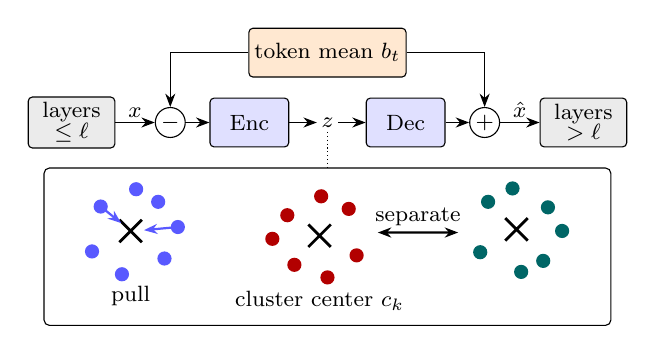
\begin{tikzpicture}[font=\footnotesize, >={Stealth[length=1.7mm]},
  box/.style={draw, rounded corners=1.5pt, minimum height=6.2mm, inner sep=2pt},
  lm/.style={box, fill=black!8, minimum width=11mm, align=center},
  ae/.style={box, fill=blue!12, minimum width=10mm},
  op/.style={draw, circle, inner sep=0pt, minimum size=3.8mm},
  pt/.style={circle, inner sep=0pt, minimum size=1.8mm},
  proto/.style={cross out, draw, line width=1pt, inner sep=0pt, minimum size=2.5mm}]
% ---- pipeline through the autoencoder
\node[lm] (lm1) {layers\\[-2pt]$\le \ell$};
\node[op, right=5mm of lm1] (minus) {$-$};
\node[ae, right=3mm of minus] (enc) {Enc};
\node[inner sep=1.5pt, right=3.5mm of enc] (z) {$z$};
\node[ae, right=3.5mm of z] (dec) {Dec};
\node[op, right=3mm of dec] (plus) {$+$};
\node[lm, right=5mm of plus] (lm2) {layers\\[-2pt]$> \ell$};
\draw[->] (lm1) -- node[above, inner sep=1.5pt] {$x$} (minus);
\draw[->] (minus) -- (enc);
\draw[->] (enc) -- (z);
\draw[->] (z) -- (dec);
\draw[->] (dec) -- (plus);
\draw[->] (plus) -- node[above, inner sep=1.5pt] {$\hat{x}$} (lm2);
% ---- token bypass
\node[box, fill=orange!18, above=4.5mm of z] (bt) {token mean $b_t$};
\draw[->] (bt.west) -| (minus.north);
\draw[->] (bt.east) -| (plus.north);
% ---- the latent with its cluster centers
\node[draw, rounded corners=2pt, below=4.5mm of z, minimum width=72mm, minimum height=20mm] (panel) {};
\draw[densely dotted] (z) -- (panel.north);
\coordinate (A) at ($(panel.center)+(-25mm,2.0mm)$);
\coordinate (B) at ($(panel.center)+(-1mm,1.4mm)$);
\coordinate (C) at ($(panel.center)+(24mm,2.2mm)$);
\foreach \dx/\dy in {-3.8/3.1, 3.5/3.7, -4.9/-2.6, 4.3/-3.5, 0.7/5.3, -1.1/-5.5, 6.0/0.5}
  \node[pt, fill=blue!65] at ($(A)+(\dx mm,\dy mm)$) {};
\foreach \dx/\dy in {-4.1/2.6, 3.7/3.4, -3.2/-3.7, 4.7/-2.5, 0.2/5.0, 1.0/-5.3, -6.0/-0.4}
  \node[pt, fill=red!70!black] at ($(B)+(\dx mm,\dy mm)$) {};
\foreach \dx/\dy in {-3.6/3.5, 4.0/2.8, -4.6/-2.9, 3.4/-4.0, -0.5/5.2, 0.6/-5.4, 5.8/-0.2}
  \node[pt, fill=teal!80!black] at ($(C)+(\dx mm,\dy mm)$) {};
\node[proto] (pa) at (A) {};
\node[proto] (pb) at (B) {};
\node[proto] (pc) at (C) {};
\draw[->, blue!65, thick] ($(A)+(6.0mm,0.5mm)$) -- ($(A)+(1.7mm,0.1mm)$);
\draw[->, blue!65, thick] ($(A)+(-3.8mm,3.1mm)$) -- ($(A)+(-1.2mm,1.0mm)$);
\draw[<->, thick] ($(B)+(7.4mm,0.4mm)$) -- node[above, inner sep=2pt] {separate} ($(C)+(-7.4mm,-0.4mm)$);
\node[anchor=north, inner sep=1pt] at ($(A)+(0,-6.6mm)$) {pull};
\node[anchor=north, inner sep=1pt] at ($(B)+(0,-6.6mm)$) {cluster center $c_k$};
\end{tikzpicture}
\caption{GeoAE. The activation of a frozen model at layer $\ell$ is encoded into a wider latent $z$ and decoded back, and the later layers run on the reconstruction. Latents are pulled toward balanced cluster centers, which are pushed apart; the mean activation of the current token, $b_t$, bypasses the autoencoder.}
\label{fig:overview}
\end{figure}

GeoAE is an autoencoder over the activations of a frozen language model at a layer, trained jointly with a codebook of $K$ clusters (Figure~\ref{fig:overview}).
Its objective adds three terms of self-supervised clustering to a reconstruction loss: a balanced assignment of latents to clusters, a pull toward the assigned cluster together with a separation term between clusters, and variance and covariance regularization of the latent. A per-token bias is routed around the AE to remove lexical signal.

\subsection{Architecture and splice}

Let $h_t \in \mathbb{R}^{d}$ be the residual stream activation at layer $\ell$ for a position whose current token is $t$, and let $x_t = (h_t - \mu) \oslash \sigma$ be its standardization, where $\mu, \sigma \in \mathbb{R}^{d}$ are the per dimension mean and standard deviation of the training activations ($\oslash$, $\odot$ denote elementwise division and multiplication).
The encoder and decoder are
\begin{align}
  z_t &= \mathrm{GELU}\big(\mathrm{BN}(W_e (x_t - b_t) + a)\big), \label{eq:ae} \\
  \hat{x}_t &= W_d\, z_t + b_t, \nonumber
\end{align}
where $z_t \in \mathbb{R}^{m}$ is the latent representation, $W_e \in \mathbb{R}^{m\times d}$ and $a \in \mathbb{R}^{m}$ are the encoder weight matrix and bias, $\mathrm{BN}$ is batch normalization \citep{ioffe2015batchnorm}, and $\mathrm{GELU}$ is the Gaussian error linear unit \citep{hendrycks2016gelu}. The decoder weight matrix $W_d \in \mathbb{R}^{d\times m}$ has no additional bias, and its columns are rescaled to unit norm after every optimizer step. The token bypass $b_t \in \mathbb{R}^{d}$ is described in \S\ref{sec:bypass}. After training, $\mathrm{BN}$ uses its running statistics, so the encoder is a fixed function of each activation.

To splice GeoAE into the model, $h_t$ is replaced by $\hat{h}_t = \sigma \odot \hat{x}_t + \mu$ at layer $\ell$. Because the decoder is linear, an edit of the latent from $z_t$ to $z_t'$ changes the activation by $\sigma \odot W_d (z_t' - z_t)$, independent of $b_t$. We apply latent edits to the original activation using this difference.



\subsection{Training Objective}

GeoAE minimizes the combined objective:
\begin{equation}
\textstyle
  \mathcal{L} = \mathcal{L}_{\mathrm{rec}}
  + \lambda_c \mathcal{L}_{\mathrm{pull}}
  + \lambda_s \mathcal{L}_{\mathrm{sep}}
  + \lambda_v \mathcal{L}_{\mathrm{var}}
  + \lambda_r \mathcal{L}_{\mathrm{cov}} 
  \label{eq:loss}
\end{equation}
where $\mathcal{L}_{\mathrm{rec}}$ is the mean squared error between $x_t$ and $\hat{x}_t$. The terms $\mathcal{L}_{\mathrm{pull}}$ and $\mathcal{L}_{\mathrm{sep}}$ are defined over clusters in a batch of $B$ latents $z_1,\dots,z_B$, with $K$ cluster centers $c_1,\dots,c_K \in \mathbb{R}^{m}$ and soft assignments $Q_{bk}\geq 0$ of latent $z_b$ to cluster $k$, where $\sum_k Q_{bk}=1$. \S~\ref{sec:assign} describes how the assignments are computed and the cluster centers are updated.

The pull term moves each latent toward the clusters it is assigned to:
\begin{equation}
\textstyle
  \mathcal{L}_{\mathrm{pull}} = \frac{1}{B m} \sum_{b=1}^{B} \sum_{k=1}^{K} Q_{bk}\, \lVert z_b - \mathrm{sg}(c_k) \rVert^2 
\end{equation}
where $\mathrm{sg}$ stops the gradient, so the loss moves the latents and not the cluster centroid.

The separation term pushes apart clusters that overlap. Let $m_k = \sum_b Q_{bk}z_b / \sum_b Q_{bk}$ be the mean of cluster $k$ in the batch, and let $r = \bigl(\frac{1}{B}\sum_{b=1}^{B}\lVert z_b-m_{k_b}\rVert^2\bigr)^{1/2}$ be the cluster radius, where $k_b=\arg\max_k Q_{bk}$ is the cluster assigned to latent $z_b$. Each pair of clusters whose means are closer than $\kappa$ radii is penalized:
\begin{equation}
\textstyle
\mathcal{L}_{\mathrm{sep}}
= \frac{1}{K(K-1)}
\sum_{k \neq k'}
\max\!\left(
0,\;
\kappa - \frac{\lVert m_k - m_{k'} \rVert}{\mathrm{sg}(r)}
\right)^2 .
\end{equation}
We set $\kappa=2$, so the term vanishes once all cluster means are at least two radii apart. Because distances are measured in units of $r$, it does not reward expanding the latent space.




The pull term can be reduced by contracting the latent space, leading to a degenerate solution. To prevent this, we use the variance and covariance regularizers from VICReg \citep{bardes2022vicreg}. The variance term, $\mathcal{L}_{\mathrm{var}} = \frac{1}{m} \sum_j \max\big(0,\, 1 - \mathrm{std}(z_{\cdot j})\big)$ prevents collapse by penalizing latent dimensions with standard deviation below one. The covariance term, $\mathcal{L}_{\mathrm{cov}} = \frac{1}{m} \sum_{j \neq l} \mathrm{Cov}(z)_{jl}^2$, discourages redundancy between latent dimensions. We set $\lambda_c=\lambda_v=1$ and $\lambda_r=0.01$, and increase $\lambda_s$ linearly from $0$ to $0.3$ during training.



% \subsection{Assignment to Clusters}
% \label{sec:assign}

% A batch of $B$ latents is assigned to the centroids by
% \begin{equation}
%   Q_{bk} = \frac{\exp\!\big( -\lVert z_b - c_k \rVert^2/\tau \big)}{\sum_{k'=1}^{K} \exp\!\big( -\lVert z_b - c_{k'} \rVert^2/\tau \big)} ,
%   \label{eq:assign}
% \end{equation}
% with a temperature $\tau$ that is annealed from 1.0 to 0.1 during training.

% The centroids are not trained by gradient descent: after each optimizer step, $c_k \leftarrow 0.9\, c_k + 0.1\, \bar{z}_k$, where $\bar{z}_k$ is the mean of the batch latents whose largest assignment is $k$ \citep[the moving-average codebook update of VQ-VAE;][]{vandenoord2017vqvae}.

\subsection{Centroid Initialization and Cluster Assignment}
\label{sec:assign}

\paragraph{Centroid initialization.} We initialize cluster centroids using density-peak selection \citep{rodriguez2014peaks}, choosing $K$ latent vectors from well-populated, distinct regions of the latent space. This encourages centroids to capture meaningful modes rather than outliers or redundant regions. During training, we use the same criterion to re-seed inactive centroids. Every $125$ steps, we move any centroid whose running usage falls below $10\%$ of its target share (Appendix~\ref{app:assignment}) to an unoccupied density peak.

\paragraph{Cluster assignment.}We compute soft assignments of batch latents to \(K\) centroids using Sinkhorn--Knopp iterations \citep{cuturi2013sinkhorn}, following SeLa and SwAV \citep{asano2020sela,caron2020swav}. Sinkhorn normalizes each latent's assignments to sum to one while encouraging aggregate centroid usage to match a target distribution \(\pi\). We initially set \(\pi\) to uniform, promoting use of all centroids and preventing assignment collapse. However, the underlying concepts need not occur equally often. Motivated by the approximately power-law frequency structure of natural language, we gradually anneal $\pi$ toward a Zipf distribution,
$\pi_k \propto \operatorname{rank}(k)^{-s}$
where centroids are ranked by running usage and $s$ increases from $0$ to $0.5$. This allows common concepts to receive more assignments while retaining a global constraint on centroid usage. Details of the relaxed Sinkhorn updates, cross-batch
potentials, and temperature schedule are provided in
Appendix~\ref{app:assignment}.

Centroids are updated by exponential moving average $c_k \leftarrow 0.9\,c_k + 0.1\,\bar{z}_k$ where \(\bar{z}_k\) is the mean of batch latents whose largest assignment is to centroid \(k\), following the VQ-VAE codebook update \citep{vandenoord2017vqvae}.




% Centroids are introduced after ten warm-up epochs that use no
% clustering loss. We initialize them with density-peak selection
% \citep{rodriguez2014density} which selects the $K$ points that are locally dense and far from any denser point. Centroids therefore start at the centers of dense regions of the
% latent space rather than at outliers. During training, a centroid that stops receiving assignments is re-seeded by the same rule. Every 125 steps, any centroid whose running usage has fallen below 10\% of its target share (Section~\ref{sec:assign}) is moved to a density peak of the current batch that no active centroid occupies.

% \subsection{Assignment to Clusters}
% \label{sec:assign}

% We compute soft assignments of batch latents to $K$ centroids
% using Sinkhorn--Knopp iterations \citep{cuturi2013sinkhorn},
% following SeLa and SwAV \citep{asano2020sela,caron2020swav}.
% Sinkhorn normalizes each latent's assignments to sum to one
% while encouraging centroid usage to match a target distribution
% $\pi$.
% We initially use a uniform target to encourage
% use of all centroids and discourage assignment collapse onto
% a small subset.

% The concepts discovered through unsupervised clustering need
% not occur equally often.
% Motivated by the power-law frequency patterns observed in
% natural language, we gradually anneal the target toward a
% Zipf distribution,
% $\pi_k \propto \operatorname{rank}(k)^{-s}$,
% where centroids are ranked by running usage and $s$ increases
% from $0$ to $0.5$.
% This allows frequently occurring concepts to receive a larger
% share of assignments while retaining a constraint on overall
% centroid usage.
% Details of the relaxed Sinkhorn updates, cross-batch
% potentials, and temperature schedule are provided in
% Appendix~\ref{app:assignment}.

% The centroids are not trained by gradient descent.
% After each optimizer step, we update them by
% \begin{equation}
%   c_k \leftarrow 0.9\,c_k + 0.1\,\bar{z}_k,
% \end{equation}
% where $\bar{z}_k$ is the mean of the batch latents whose
% largest assignment is to centroid $k$.
% This follows the moving-average codebook update of VQ-VAE
% \citep{vandenoord2017vqvae}.
% \subsection{Assignment to Clusters}
% \label{sec:assign}

% A batch of $B$ latents is assigned to the centroids by
% \begin{equation}
%   Q_{bk} = \exp\!\big( -\lVert z_b - c_k \rVert^2/\tau + f_b + g_k \big),
%   \label{eq:assign}
% \end{equation}
% with temperature $\tau$.
% The potentials $f_b$ normalize each row to one, $\sum_k Q_{bk} = 1$, and the potentials $g_k$ move each column sum $\sum_b Q_{bk}$ toward $B \pi_k$, where $\pi_k$ is the target share of the batch assigned to centroid $k$ ($\sum_k \pi_k = 1$).
% We compute $f$ and $g$ with three Sinkhorn--Knopp iterations \citep{cuturi2013sinkhorn}, as in SeLa and SwAV \citep{asano2020sela,caron2020swav}, with two changes: each update of $g$ is scaled by $\rho = 0.6$, which relaxes the column constraint as in unbalanced optimal transport \citep{chizat2018scaling}, and $g$ is carried across batches at rate $\eta = 0.05$, so that balance holds across batches.
% The target $\pi$ is annealed from uniform, $\pi_k = 1/K$, toward a Zipf law over the centroids ranked by running usage, $\pi_k \propto \mathrm{rank}(k)^{-s}$ with $s$ rising from 0 to 0.5, and $\tau$ is annealed from 1.0 to 0.1.

% The centroids are not trained by gradient descent: after each optimizer step, $c_k \leftarrow 0.9\, c_k + 0.1\, \bar{z}_k$, where $\bar{z}_k$ is the mean of the batch latents whose largest assignment is $k$ \citep[the moving-average codebook update of VQ-VAE;][]{vandenoord2017vqvae}.


% \subsection{Token bypass}
% \label{sec:bypass}

% Residual stream activations retain substantial information about token identity across layers \citep{rizwan2026persistent}. This lexical signal can dominate the geometry of the learned representation, causing tokens with the same identity to cluster together even when they appear in different contexts. We therefore introduce a token specific bypass that captures the average activation associated with each token type.

% For each token type $t$, we collect all occurrences of $t$ in the training data and average their standardized activations:
% \begin{equation}
%   b_t =
%   \frac{n_t}{n_t + 30}
%   \cdot
%   \frac{1}{n_t}
%   \sum_{i\,:\,t_i=t} x_i ,
%   \label{eq:bypass}
% \end{equation}
% where $n_t$ is the number of times token $t$ appears in the training data, $t_i$ is the token at occurrence $i$, and $x_i$ is its standardized activation. The factor $n_t/(n_t+30)$ shrinks the estimate toward zero for rare tokens, and we set $b_t=0$ for tokens observed fewer than ten times.

% For Llama-3.2-3B, the bypass covers 49,664 token types and 98.5\% of token occurrences in the training data. We subtract $b_t$ before the encoder and add it back after the decoder (Eq.~\ref{eq:ae}). This preserves the average contribution associated with token identity while encouraging the latent representation to capture variation beyond it. During latent interventions, the bypass remains fixed because the identity of the current token does not change.

% the closest prior design.

\subsection{Token bypass}
\label{sec:bypass}

Residual stream activations retain substantial information
about token identity across layers
\citep{rizwan2026persistent}.
This lexical signal can encourage occurrences of the same
token to cluster together despite differences in context.
We therefore introduce a fixed token bypass that captures
the average activation associated with each token type,
allowing the encoder to focus on variation around this
baseline.

For each token type $t$, we estimate its baseline from
standardized training activations:
\begin{equation}
  b_t = \frac{n_t}{n_t+\lambda_b}\,\bar{x}_t,
  \qquad
  \bar{x}_t = \frac{1}{n_t}\sum_{i:t_i=t} x_i,
  \label{eq:bypass}
\end{equation}
where $n_t$ counts training occurrences of $t$ and
$\lambda_b$ controls shrinkage toward zero.
Shrinkage reduces the influence of noisy means estimated
from few occurrences.
We use $\lambda_b=30$, so a token observed 30 times retains
half its empirical mean, while frequent tokens retain
nearly their full mean.
Tokens observed fewer than ten times receive $b_t=0$.

We subtract $b_t$ before the encoder and add it back after
the decoder (Eq.~\ref{eq:ae}).
This preserves the baseline contribution in the reconstruction
while encouraging the latent representation to capture
variation beyond it.

Appendix~\ref{app:bypass} gives further details and the bypass statistics of each model.

\subsection{Training}
\label{sec:training}

GeoAE is trained for 50 epochs with AdamW \citep{loshchilov2019adamw} using a batch size of 32{,}768 activations. We use a staged training schedule so that clustering is introduced only after the autoencoder has learned a faithful representation. Epochs 1-5 optimize reconstruction alone, and epochs 6-10 additionally include the variance and covariance regularizers. At epoch 11, we initialize the cluster centers at density peaks in the latent space \citep{rodriguez2014peaks} and activate the pull and separation losses for the remainder of training. Appendix~\ref{app:hyper} provides complete training details and hyperparameters, while Appendix~\ref{app:ablations} presents ablations evaluating the effect of removing the token bypass and varying the latent width and number of clusters.







\section{Experimental Setup}
\label{sec:setup}

% Table rows generated by eval_out/paper_geometry_table.py from the result files.
\begin{table*}[t]
\centering
\small
\setlength{\tabcolsep}{5pt}
\begin{tabular}{@{}l rr c rrr c rr@{}}
\toprule
 & \multicolumn{2}{c}{Llama-3.2-3B} && \multicolumn{3}{c}{Gemma~3 4B} && \multicolumn{2}{c}{Qwen2.5-3B} \\
\cmidrule(lr){2-3}\cmidrule(lr){5-7}\cmidrule(l){9-10}
 & Base & GeoAE && Base & SAE & GeoAE && Base & GeoAE \\
\midrule
\multicolumn{10}{@{}l}{\emph{Cluster geometry}} \\
\quad Calinski-Harabasz $\uparrow$ & $197.6$ & $\mathbf{673.7}$ && $124.4$ & $442.6$ & $\mathbf{595.9}$ && $149.8$ & $\mathbf{664.0}$ \\
\quad Davies-Bouldin $\downarrow$ & $4.46$ & $\mathbf{3.36}$ && $4.63$ & $\mathbf{3.37}$ & $3.56$ && $4.15$ & $\mathbf{3.50}$ \\
\quad Silhouette $\uparrow$ & ${-}0.024$ & $\mathbf{{-}0.009}$ && ${-}0.146$ & $\mathbf{{-}0.012}$ & ${-}0.028$ && ${-}0.073$ & $\mathbf{{-}0.048}$ \\
\quad Within-cluster variance (\%) $\downarrow$ & $72$ & $\mathbf{43}$ && $80$ & $53$ & $\mathbf{46}$ && $77$ & $\mathbf{43}$ \\
\addlinespace[2pt]
\multicolumn{10}{@{}l}{\emph{Reconstruction of the activations}} \\
\quad Variance explained (\%) $\uparrow$ & -- & $96.5$ && -- & $62.7$ & $\mathbf{96.2}$ && -- & $97.1$ \\
\quad Normalized MSE $\downarrow$ & -- & $0.035$ && -- & $0.373$ & $\mathbf{0.038}$ && -- & $0.029$ \\
\addlinespace[2pt]
\multicolumn{10}{@{}l}{\emph{Faithfulness of the spliced model}} \\
\quad MMLU accuracy (\%) $\uparrow$ & $56.2$ & $55.0$ && $55.3$ & $\mathbf{54.3}$ & $53.0$ && $65.1$ & $64.6$ \\
\quad WikiText-2 perplexity $\downarrow$ & $7.83$ & $8.56$ && $7.39$ & $13.67$ & $\mathbf{8.26}$ && $8.03$ & $8.67$ \\
\bottomrule
\end{tabular}
\caption{Last-layer cluster geometry, reconstruction, and faithfulness ($K=2{,}000$). Base: $k$-means on standardized residual activations; GeoAE: token-bypass latents with their centroids; SAE: $k$-means on pretrained Gemma Scope SAE codes (16k features). Geometry uses 1M activations and Euclidean distances in each space’s own coordinates.}
\label{tab:geometry}
\end{table*}


\paragraph{Models and training data.}
We train GeoAEs on residual stream activations from the output of the final transformer block of three pretrained language models from different families. The models are Llama 3.2 3B \citep{meta2024llama}, Gemma 3 4B \citep{gemma2025gemma}, and Qwen2.5 3B \citep{qwen2024qwen2}. For each model, we use a corpus mixture resembling its pretraining data, including web text, Wikipedia, code, mathematics, and non-English text. During training, we sample 64 token positions from each document and compute the GeoAE objective on the corresponding final layer activations. Across documents, this yields 10M activations, of which 5\% are held out for validation (Appendix~\ref{app:data}).
% We train GeoAEs on the residual stream after the final block of three pretrained language models from different families. The models include Llama-3.2-3B \citep{meta2024llama} Gemma~3 4B \citep{gemma2025gemma}, and Qwen2.5-3B \citep{qwen2024qwen2}. For each model, we collect 10M activations from a mixture that resembles the pretraining corpus (web text, Wikipedia, code, mathematics and non-English text) sampling 64 token positions per document, and hold out 5\% for validation (Appendix~\ref{app:data}).

\paragraph{GeoAE and baselines.}


We use the same training procedure for all three models (\S\ref{sec:method}).
The latent is twice as wide as the residual stream, giving $m = 6{,}144$, $5{,}120$, and $4{,}096$ for Llama, Gemma, and Qwen, and the number of clusters is $K = 2{,}000$ for all models. For each model, we train two GeoAE variants that differ only in the token bypass. The bypass variant is used for geometry, faithfulness, sequence-level structure, and control, while the no-bypass variant retains token identity in the latent and is used for token-level structure.


Our baseline is standard $k$-means clustering \citep{lloyd1982least} with the same $K$ and initialization, applied to the standardized residual stream of each model. For sequence-level comparisons, we apply the same token mean subtraction before $k$ means. This controls for the removal of token identity and isolates the contribution of the learned encoder. In the control experiments (\S\ref{sec:control}), the baseline applies the corresponding edit directly to the residual stream. For Gemma, we also compare with the pretrained Gemma Scope~2 SAE of the same layer \citep[16k JumpReLU features;][]{mcdougall2025gemma}, clustering its code vectors with $k$-means at the same $K$.

% Our baseline is standard $k$-means \citep{lloyd1982least} with the same $K$ and initialization, applied to the standardized residual stream of each model.
% For sequence-level comparisons with the bypass GeoAE, we instead apply $k$-means to the token-removed residual stream, obtained by subtracting the same token-specific means that the bypass uses. This baseline removes token identity without an encoder and therefore isolates the contribution of the encoder.
% In the control experiments (\S\ref{sec:control}), the baseline is the same edit applied to the residual stream.




% \paragraph{GeoAE and baselines.}
% All models share one recipe (\S\ref{sec:method}; hyperparameters in Appendix~\ref{app:hyper}): a latent twice as wide as the residual stream ($d = 6{,}144$, $5{,}120$ and $4{,}096$) and $K = 2{,}000$ cluster centers.
% We train two variants per model that differ only in the token bypass: the \emph{bypass} GeoAE, used for geometry, faithfulness, sequence-level structure and control, and a \emph{no-bypass} GeoAE, which keeps token identity in the latent and is used for token-level structure.
% The reference in every comparison is $k$-means with the same $K$ and initialization on the model's own standardized residual stream (balanced as in \S\ref{sec:assign} for geometry, plain \citep{lloyd1982least} for concept alignment; the two have nearly the same geometry, Appendix~\ref{app:ablations}).
% Because the bypass removes a per-token mean before encoding, the sequence-level comparisons use $k$-means on the \emph{token-removed} residual stream, which subtracts the same means and has no encoder; this isolates what the encoder adds.
% On Gemma we also compare with the pretrained Gemma Scope~2 SAE of the same layer \citep[16k JumpReLU features;][]{mcdougall2025gemma}, clustering its code vectors with $k$-means at the same $K$.

\begin{table*}[t]
  \centering
  \scriptsize
  \setlength{\tabcolsep}{2.2pt}
  \resizebox{\textwidth}{!}{%
  \begin{tabular}{@{}l
                  ccc ccc
                  ccc ccc ccc
                  ccc ccc@{}}
    \toprule
    & \multicolumn{6}{c}{Llama-3.2-3B, layer 27}
    & \multicolumn{9}{c}{Gemma~3 4B, layer 33}
    & \multicolumn{6}{c}{Qwen2.5-3B, layer 35} \\
    \cmidrule(lr){2-7}
    \cmidrule(lr){8-16}
    \cmidrule(l){17-22}

    & \multicolumn{3}{c}{$k$-means}
    & \multicolumn{3}{c}{GeoAE}
    & \multicolumn{3}{c}{$k$-means}
    & \multicolumn{3}{c}{SAE}
    & \multicolumn{3}{c}{GeoAE}
    & \multicolumn{3}{c}{$k$-means}
    & \multicolumn{3}{c}{GeoAE} \\

    & H & C & NMI
    & H & C & NMI
    & H & C & NMI
    & H & C & NMI
    & H & C & NMI
    & H & C & NMI
    & H & C & NMI \\
    \midrule

    Surface form (7)
    & .680 & .149 & .244
    & \textbf{.765} & .157 & .261
    & .641 & .200 & .305
    & .487 & .190 & .273
    & \textbf{.707} & .227 & .343
    & .660 & .167 & .267
    & \textbf{.764} & .169 & .277 \\

    POS, Penn (44)
    & .609 & .306 & .407
    & \textbf{.730} & .346 & .469
    & .404 & .289 & .337
    & .245 & .217 & .230
    & \textbf{.507} & .372 & .429
    & .600 & .335 & .430
    & \textbf{.746} & .362 & .487 \\

    Entity type (9)
    & .458 & .078 & .134
    & \textbf{.516} & .088 & .150
    & .357 & .075 & .124
    & .255 & .066 & .105
    & \textbf{.388} & .087 & .142
    & .468 & .081 & .138
    & \textbf{.528} & .087 & .150 \\

    \bottomrule
  \end{tabular}%
  }
  \caption{
  Token-level structure with $K=2{,}000$ clusters.
  H, C, and NMI denote homogeneity, completeness, and normalized mutual information.
  GeoAE is evaluated without the token bypass against $k$-means on the same residual stream and, for Gemma, against $k$-means on representations from the pretrained Gemma Scope SAE (16k features).
  Bold marks the highest homogeneity for each model.
  Evaluation includes rows belonging to clusters containing at least ten examples from the task.
  }
  \label{tab:token}
\end{table*}

% \begin{table*}[t]
%   \centering
%   \scriptsize
%   \setlength{\tabcolsep}{4.5pt}
%   \begin{tabular}{@{}l cc c ccc c cc@{}}
%     \toprule
%     & \multicolumn{2}{c}{Llama-3.2-3B, layer 27} && \multicolumn{3}{c}{Gemma~3 4B, layer 33} && \multicolumn{2}{c}{Qwen2.5-3B, layer 35} \\
%     \cmidrule(lr){2-3} \cmidrule(lr){5-7} \cmidrule(l){9-10}
%     Task & $k$-means & GeoAE && $k$-means & SAE & GeoAE && $k$-means & GeoAE \\
%     \midrule
%     Surface form (7) & .680/.149/.244 & \textbf{.765}/.157/.261 &  & .641/.200/.305 & .487/.190/.273 & \textbf{.707}/.227/.343 &  & .660/.167/.267 & \textbf{.764}/.169/.277 \\
%     POS, Penn (44) & .609/.306/.407 & \textbf{.730}/.346/.469 &  & .404/.289/.337 & .245/.217/.230 & \textbf{.507}/.372/.429 &  & .600/.335/.430 & \textbf{.746}/.362/.487 \\
%     Entity type (9) & .458/.078/.134 & \textbf{.516}/.088/.150 &  & .357/.075/.124 & .255/.066/.105 & \textbf{.388}/.087/.142 &  & .468/.081/.138 & \textbf{.528}/.087/.150 \\
%     \bottomrule
%   \end{tabular}
%   \caption{Token-level structure ($K = 2{,}000$ clusters each): the GeoAE without the token bypass against plain $k$-means on the same residual stream and, on Gemma, against plain $k$-means on the codes of the pretrained Gemma Scope SAE (16k features). Cells give homogeneity / completeness / NMI of the clusters against the task's labels (class counts in brackets); bold marks the highest homogeneity per model. Each space is scored on the rows that fall in its own clusters holding at least ten of the task's rows (97--98\% of rows for part of speech).}
%   \label{tab:token}
% \end{table*}

\begin{table*}[t]
  \centering
  \scriptsize
  \setlength{\tabcolsep}{2.2pt}
  \resizebox{\textwidth}{!}{%
  \begin{tabular}{@{}l
                  ccc ccc
                  ccc ccc ccc
                  ccc ccc@{}}
    \toprule
    & \multicolumn{6}{c}{Llama-3.2-3B, layer 27}
    & \multicolumn{9}{c}{Gemma~3 4B, layer 33}
    & \multicolumn{6}{c}{Qwen2.5-3B, layer 35} \\
    \cmidrule(lr){2-7}
    \cmidrule(lr){8-16}
    \cmidrule(l){17-22}

    & \multicolumn{3}{c}{$k$-means}
    & \multicolumn{3}{c}{GeoAE}
    & \multicolumn{3}{c}{$k$-means}
    & \multicolumn{3}{c}{SAE}
    & \multicolumn{3}{c}{GeoAE}
    & \multicolumn{3}{c}{$k$-means}
    & \multicolumn{3}{c}{GeoAE} \\

    & H & C & NMI
    & H & C & NMI
    & H & C & NMI
    & H & C & NMI
    & H & C & NMI
    & H & C & NMI
    & H & C & NMI \\
    \midrule

    \multicolumn{22}{@{}l}{\emph{Probes (last token of each text)}} \\

    Domain (3)
    & .970 & .367 & .532
    & \textbf{.980} & .322 & .485
    & .760 & .261 & .389
    & .852 & .245 & .381
    & \textbf{.866} & .239 & .374
    & .956 & .356 & .518
    & \textbf{.969} & .279 & .433 \\

    AG News (4)
    & .446 & .239 & .312
    & \textbf{.463} & .216 & .295
    & .172 & .118 & .140
    & .040 & .028 & .033
    & \textbf{.360} & .176 & .236
    & .541 & .232 & .325
    & \textbf{.653} & .269 & .381 \\

    DBpedia-14 (14)
    & .692 & .703 & .698
    & \textbf{.811} & .609 & .696
    & .389 & .370 & .379
    & .112 & .167 & .134
    & \textbf{.604} & .468 & .528
    & .605 & .613 & .609
    & \textbf{.628} & .516 & .566 \\

    20 Newsgroups (20)
    & .084 & .108 & .094
    & \textbf{.152} & .147 & .150
    & .058 & .096 & .073
    & .061 & .085 & .071
    & \textbf{.146} & .164 & .154
    & .105 & .132 & .117
    & \textbf{.246} & .233 & .239 \\

    Jigsaw toxicity (2)
    & .171 & .037 & .061
    & \textbf{.225} & .050 & .082
    & .234 & .068 & .106
    & .159 & .050 & .076
    & \textbf{.264} & .069 & .110
    & .159 & .043 & .068
    & \textbf{.225} & .060 & .095 \\

    \midrule
    \multicolumn{22}{@{}l}{\emph{FineWeb-Atlas (last word of each chunk)}} \\

    14 topics (3 draws)
    & .189 & .114 & .141
    & \textbf{.295} & .165 & .210
    & .286 & .174 & .215
    & .207 & .117 & .148
    & \textbf{.341} & .192 & .244
    & .188 & .128 & .152
    & \textbf{.366} & .216 & .270 \\

    \bottomrule
  \end{tabular}%
  }
  \caption{
  % Sequence-level structure with $K=2{,}000$ clusters.
  % H, C, and NMI denote homogeneity, completeness, and normalized mutual information.
  % The token-bypass GeoAE is compared with $k$-means on the token-removed residual stream, which subtracts the same per-token means and has no encoder, and on Gemma with $k$-means on pretrained Gemma Scope SAE codes.
  % Probes read the last token of each text, while FineWeb-Atlas reads the last word of chunks containing exactly one of 14 topic concepts and averages results over three draws.
  % $^{*}$ indicates that the document-bootstrap 95\% confidence interval of the homogeneity difference excludes zero in every draw.
  % $k$-means and GeoAE are evaluated on the same rows whose clusters contain at least ten scored examples in both spaces (41--84\% of rows).
  % For the SAE comparison, GeoAE homogeneity on the matched rows is .922, .368, .595, .142, .255, and .344 from top to bottom.%
  Sequence-level structure with $K=2{,}000$ clusters. H, C, and NMI denote homogeneity, completeness, and normalized mutual information. Token-bypass GeoAE is compared with $k$-means on residual activations after subtracting the same per-token means (without an encoder) and, for Gemma, on pretrained Gemma Scope SAE codes.}
  \label{tab:seq}
\end{table*}

% \begin{table*}[t]
%   \centering
%   \scriptsize
%   \setlength{\tabcolsep}{4.5pt}
%   \begin{tabular}{@{}l cc c ccc c cc@{}}
%     \toprule
%     & \multicolumn{2}{c}{Llama-3.2-3B, layer 27} && \multicolumn{3}{c}{Gemma~3 4B, layer 33} && \multicolumn{2}{c}{Qwen2.5-3B, layer 35} \\
%     \cmidrule(lr){2-3} \cmidrule(lr){5-7} \cmidrule(l){9-10}
%     Task & $k$-means & GeoAE && $k$-means & SAE & GeoAE && $k$-means & GeoAE \\
%     \midrule
%     \multicolumn{10}{@{}l}{\emph{Probes (last token of each text)}} \\
%     Domain (3) & .970/.367/.532 & \textbf{.980}/.322/.485 &  & .760/.261/.389 & .852/.245/.381 & \textbf{.866}/.239/.374 &  & .956/.356/.518 & \textbf{.969}/.279/.433 \\
%     AG News (4) & .446/.239/.312 & \textbf{.463}/.216/.295 &  & .172/.118/.140 & .040/.028/.033 & \textbf{.360}/.176/.236 &  & .541/.232/.325 & \textbf{.653}/.269/.381 \\
%     DBpedia-14 (14) & .692/.703/.698 & \textbf{.811}/.609/.696 &  & .389/.370/.379 & .112/.167/.134 & \textbf{.604}/.468/.528 &  & .605/.613/.609 & \textbf{.628}/.516/.566 \\
%     20 Newsgroups (20) & .084/.108/.094 & \textbf{.152}/.147/.150 &  & .058/.096/.073 & .061/.085/.071 & \textbf{.146}/.164/.154 &  & .105/.132/.117 & \textbf{.246}/.233/.239 \\
%     Jigsaw toxicity (2) & .171/.037/.061 & \textbf{.225}/.050/.082 &  & .234/.068/.106 & .159/.050/.076 & \textbf{.264}/.069/.110 &  & .159/.043/.068 & \textbf{.225}/.060/.095 \\
%     \midrule
%     \multicolumn{10}{@{}l}{\emph{FineWeb-Atlas (last word of each chunk)}} \\
%     14 topics (3 draws) & .189/.114/.141 & \textbf{.295}$^{*}$/.165/.210 &  & .286/.174/.215 & .207/.117/.148 & \textbf{.341}$^{*}$/.192/.244 &  & .188/.128/.152 & \textbf{.366}$^{*}$/.216/.270 \\
%     \bottomrule
%   \end{tabular}
%   \caption{Sequence-level structure ($K = 2{,}000$ clusters each): the token-bypass GeoAE against plain $k$-means on the token-removed residual stream, which subtracts the same per-token means and has no encoder. Cells as in Table~\ref{tab:token}. Probes read the last token of each text; FineWeb-Atlas reads the last word of each chunk, on chunks carrying exactly one of 14 topic concepts, averaged over three draws; $^{*}$the document-bootstrap 95\% interval of the homogeneity difference excludes zero in every draw. $k$-means and GeoAE are scored on the same rows, those whose cluster holds at least ten scored rows in both spaces (41--84\% of rows). SAE: plain $k$-means on the Gemma Scope codes, scored on the rows kept for both the SAE and GeoAE, on which GeoAE has homogeneity .922, .368, .595, .142, .255 and .344 (top to bottom).}
%   \label{tab:seq}
% \end{table*}

\paragraph{Evaluation data.}
We compare clusters with labels at two grains.
\emph{Token-level} tasks label every token of a sentence: its surface form (seven orthographic classes), its part of speech (44 Penn Treebank tags; \citealp{marcus1993penntreebank}) and its entity type (the nine coarse types of Few-NERD; \citealp{ding2021fewnerd}), with 80k labeled tokens per task.
\emph{Sequence-level} tasks label a text, which we read at its last token: domain (code, mathematics or prose; \citealp{husain2019codesearchnet,zhang2024stackmathqa,wikimedia2023wikipedia}), AG News and DBpedia-14 topics \citep{zhang2015datasets}, 20 Newsgroups \citep{rennie2008newsgroups} and Jigsaw toxicity \citep{jigsaw2018toxicity}, with 2.5k--3.5k texts each.
FineWeb-Atlas \citep{monson2026finewebatlas} annotates web text with 16{,}790 concepts; we draw 14 topic concepts three times and keep the chunks that carry exactly one of them. For control experiments, we cast DBpedia-14, AG News, Bias in Bios \citep[27 professions;][]{dearteaga2019biasbios}, 20 Newsgroups and the FineWeb-Atlas topics as few-shot classification.

\paragraph{Metrics.}
\emph{Geometry.} We assign each sample representation to its nearest centroid and report four complementary measures of cluster structure. The Calinski--Harabasz (CH) index compares how spread out the cluster centroids are with how spread out representations are around their assigned centroids, with higher values indicating tighter and better separated clusters \citep{calinski1974dendrite}. The Davies--Bouldin index compares each cluster with its most similar neighboring cluster, with lower values indicating better separation \citep{davies1979cluster}. The silhouette score compares a representation's distance to its assigned cluster with its distance to neighboring clusters, with higher values indicating clearer cluster membership \citep{rousseeuw1987silhouettes}. We also report the fraction of total variance that lies within clusters, where lower values indicate that more of the variation separates clusters rather than occurring within them. All metrics use Euclidean distances in the representation space under evaluation.

\emph{Faithfulness.} We replace the layer's output with its reconstruction and report zero-shot accuracy on 2{,}000 MMLU test questions \citep{hendrycks2021measuring} and perplexity on the WikiText-2 test set \citep{merity2017pointer}.


\emph{Concept alignment.} For label concept alignment to clusters, we report homogeneity \citep{rosenberg2007vmeasure}, $h = 1 - H(\text{label} \mid \text{cluster}) / H(\text{label})$, which reaches 1 when every cluster holds a single label, together with completeness and NMI.

\emph{Control.} To showcase control performance, we steer away from a target concept towards auxiliary concepts and measure the effect on documents the unedited model classifies correctly. We report the accuracy drop on documents of the target concept (target drop, higher is better), the accuracy drop on documents of the auxiliary concepts (collateral, lower is better), and selectivity, the target drop minus the collateral, which is high only when an edit removes the target concept while leaving the others intact.


% \section{Geometry and Faithfulness}
% \label{sec:geometry}

% \begin{table*}[t]
% \centering
% \small
% \setlength{\tabcolsep}{4pt}
% % Generated by eval_out/paper_control_plain_table.py (plain steering, alpha 0.5, accuracy points, plain means over concepts).
% \begin{tabular}{@{}l rrrr rrrr rrr@{}}
% \toprule
%  & \multicolumn{4}{c}{Target drop $\uparrow$} & \multicolumn{4}{c}{Collateral $\downarrow$} & \multicolumn{3}{c}{$\Delta$ Sel.\ vs.\ Base $\uparrow$} \\
% \cmidrule(lr){2-5}\cmidrule(lr){6-9}\cmidrule(l){10-12}
% Dataset & Base & SAE & SAE$_{1}$ & GeoAE & Base & SAE & SAE$_{1}$ & GeoAE & SAE & SAE$_{1}$ & GeoAE \\
% \midrule
% \multicolumn{12}{@{}l}{\textit{Llama-3.2-3B}} \\
% \quad DBpedia-14 & $72.3$ & -- & -- & $66.9$ & $25.6$ & -- & -- & $19.4$ & -- & -- & $+0.9$ \\
% \quad Bias in Bios & $58.5$ & -- & -- & $63.4$ & $7.2$ & -- & -- & $7.5$ & -- & -- & $+4.6$ \\
% \quad AG News & $75.7$ & -- & -- & $76.0$ & $6.9$ & -- & -- & $0.6$ & -- & -- & $+6.5$ \\
% \quad Emotion & $53.2$ & -- & -- & $55.8$ & $4.0$ & -- & -- & $4.2$ & -- & -- & $+2.4$ \\
% \quad 20NG & $61.1$ & -- & -- & $61.0$ & $8.8$ & -- & -- & $9.2$ & -- & -- & $-0.5$ \\
% \quad FineWeb-Atlas & $70.7$ & -- & -- & $69.3$ & $9.2$ & -- & -- & $9.0$ & -- & -- & $-1.1$ \\
% \quad \emph{All (105 concepts)} & $65.4$ & -- & -- & $65.7$ & $10.1$ & -- & -- & $9.2$ & -- & -- & $+1.2$ \\
% \addlinespace[2pt]
% \multicolumn{12}{@{}l}{\textit{Gemma 3 4B}} \\
% \quad DBpedia-14 & $61.4$ & $80.2$ & $21.4$ & $71.5$ & $7.7$ & $7.2$ & $2.1$ & $9.3$ & $\mathbf{+19.2}$ & $-34.3$ & $+8.5$ \\
% \quad Bias in Bios & $37.4$ & $53.5$ & $23.2$ & $53.2$ & $2.5$ & $8.9$ & $3.0$ & $3.9$ & $+9.7$ & $-14.6$ & $\mathbf{+14.4}$ \\
% \quad AG News & $59.7$ & $60.5$ & $11.6$ & $64.0$ & $0.0$ & $1.2$ & $0.0$ & $0.3$ & $-0.4$ & $-48.1$ & $\mathbf{+4.0}$ \\
% \quad Emotion & $45.9$ & $50.8$ & $21.0$ & $55.2$ & $5.4$ & $3.3$ & $1.5$ & $5.6$ & $+6.9$ & $-20.9$ & $\mathbf{+9.1}$ \\
% \quad 20NG & $63.8$ & $61.9$ & $22.9$ & $66.1$ & $9.0$ & $9.3$ & $1.9$ & $8.5$ & $-2.2$ & $-33.9$ & $\mathbf{+2.7}$ \\
% \quad FineWeb-Atlas & $59.7$ & $68.9$ & $19.2$ & $71.6$ & $7.3$ & $8.5$ & $1.8$ & $8.8$ & $+8.0$ & $-35.0$ & $\mathbf{+10.4}$ \\
% \quad \emph{All (97 concepts)} & $53.3$ & $64.0$ & $20.9$ & $64.5$ & $5.8$ & $7.9$ & $2.1$ & $6.9$ & $+8.5$ & $-28.8$ & $\mathbf{+10.0}$ \\
% \addlinespace[2pt]
% \multicolumn{12}{@{}l}{\textit{Qwen2.5-3B}} \\
% \quad DBpedia-14 & $46.9$ & -- & -- & $60.4$ & $9.0$ & -- & -- & $8.0$ & -- & -- & $+14.5$ \\
% \quad Bias in Bios & $55.8$ & -- & -- & $62.2$ & $6.9$ & -- & -- & $8.6$ & -- & -- & $+4.7$ \\
% \quad AG News & $66.1$ & -- & -- & $74.1$ & $0.9$ & -- & -- & $1.6$ & -- & -- & $+7.4$ \\
% \quad Emotion & $54.6$ & -- & -- & $55.6$ & $4.2$ & -- & -- & $5.4$ & -- & -- & $-0.2$ \\
% \quad 20NG & $68.3$ & -- & -- & $71.9$ & $14.3$ & -- & -- & $15.3$ & -- & -- & $+2.6$ \\
% \quad FineWeb-Atlas & $61.1$ & -- & -- & $70.2$ & $9.2$ & -- & -- & $11.2$ & -- & -- & $+7.1$ \\
% \quad \emph{All (103 concepts)} & $58.9$ & -- & -- & $66.4$ & $8.8$ & -- & -- & $10.1$ & -- & -- & $+6.2$ \\
% \bottomrule
% \end{tabular}
% \caption{Steering away from a concept ($\alpha = 0.5$) in the residual stream (Base), in the GeoAE latent and, on Gemma, in the codes of the pretrained Gemma Scope SAE, either all features (SAE) or only the single feature that best separates the concept (SAE$_1$). Documents are true positives of every model compared in a row (up to 100 per class). Target drop: accuracy lost on the edited concept's documents; Collateral: accuracy lost on documents of other classes; $\Delta$ Sel.: selectivity (target drop minus collateral) relative to Base; on Gemma the most selective space is in bold. Accuracy points, means over concepts; FineWeb-Atlas pools the topics of three draws. Classes with fewer than 20 true-positive documents are dropped (Appendix~\ref{app:control}).}
% \label{tab:control}
% \end{table*}


% \paragraph{GeoAE separates the clusters.}
% Table~\ref{tab:geometry} compares the clusters of the residual stream with those of the GeoAE latent.
% In the residual stream, 71--80\% of the variance lies within clusters; in the latent this share falls to 43--46\%.
% Accordingly, the Calinski--Harabasz index rises $3.4\times$ on Llama, $4.7\times$ on Gemma and $4.3\times$ on Qwen, and the Davies--Bouldin index and the silhouette improve in all three models.
% The separation is not obtained by abandoning part of the codebook: more than 99\% of the 2{,}000 cluster centers remain in use.
% Many pairs of clusters also lie along one direction at different magnitudes and can be edited separately (Appendix~\ref{app:ranges}).

% \paragraph{The model keeps working on the reshaped space.}
% With the GeoAE reconstruction spliced in, the models retain 95.3--99.2\% of their MMLU accuracy, and WikiText-2 perplexity rises by 8--12\%.

% \paragraph{Comparison with the SAE.}
% The code space of the Gemma Scope SAE, clustered in the same way, is also better separated than the residual stream: GeoAE leaves less variance within clusters (45.6\% against 53.0\%), and the SAE has slightly better Davies--Bouldin and silhouette values.
% The SAE keeps more MMLU accuracy (54.3 against 52.6; in a paired run on the same questions the difference is not significant, McNemar $p = 0.21$), but it raises perplexity from 7.39 to 13.67, seven times the increase caused by GeoAE.

\section{Geometry and Faithfulness}
\label{sec:geometry}

\paragraph{Cluster geometry.}
Across three models, GeoAE reduces the fraction of variance
within clusters from 72--80\% to 43--46\% and increases the
Calinski--Harabasz index by $3.4$--$4.8\times$
(Table~\ref{tab:geometry}).
Davies--Bouldin and silhouette likewise indicate more compact and better separated clusters.
Showcasing improved clustering structure across all metrics.

\paragraph{Reconstruction faithfulness.}
On held-out activations, GeoAE explains 96.2--97.1\% of the variance across the three models (normalized MSE
0.029-0.038).
Replacing residual activations with GeoAE reconstructions
retains 95.8--99.2\% of baseline MMLU accuracy and increases WikiText-2 perplexity by 8-12\%.
For comparison, the Gemma Scope SAE with 16k features explains only 62.7\% of the variance
(normalized MSE 0.373, against 0.038 for GeoAE) and increases perplexity by 85\%.


\paragraph{Comparison with Gemma Scope.} Under the same clustering procedure, GeoAE achieves a higher Calinski--Harabasz score ($595.9$ vs.\ $442.6$) and a lower within-cluster variance share ($46\%$ vs.\ $53\%$) than the Gemma Scope SAE. The SAE also reconstructs the original activations substantially less accurately, explaining only $62.7\%$ of their variance with a normalized MSE of $0.373$, compared with $96.2\%$ and $0.038$ for GeoAE. The SAE obtains slightly better Davies-Bouldin ($3.37$ vs.\ $3.56$) and silhouette ($-0.012$ vs.\ $-0.028$) scores. It also degrades language modeling more severely, increasing WikiText-2 perplexity from $7.39$ to $13.67$, compared with $8.26$ under GeoAE. The SAE retains higher MMLU accuracy ($54.3\%$ vs.\ $53.0\%$), although a paired evaluation finds no significant difference ($p=0.21$).

% \section{Concept Alignment}
% \label{sec:alignment}

% \paragraph{Token-level structure.}
% Without the bypass, GeoAE clusters are more homogeneous than $k$-means clusters of the same residual stream on every task and model (Table~\ref{tab:token}).
% For part of speech, homogeneity rises from .61 to .73 on Llama, from .40 to .51 on Gemma and from .60 to .75 on Qwen.
% Completeness rises in all nine comparisons as well, so the clusters do not become purer by splitting classes more finely.

% \paragraph{Sequence-level structure.}
% With the bypass, the latent describes the context instead of the current token, and its clusters group whole texts (Table~\ref{tab:seq}).
% Read at the last token, GeoAE clusters are more homogeneous than clusters of the token-removed residual stream in all 15 task--model pairs.
% Since both spaces have the token means removed, this difference is the contribution of the encoder.
% On FineWeb-Atlas, where the 14 labels are drawn from 16{,}790 concepts, homogeneity rises from .19 to .29 on Llama, from .29 to .34 on Gemma and from .19 to .37 on Qwen; the interval of the difference excludes zero in every draw, and completeness rises as well.
% On the probes the gain is one of purity: completeness and NMI rise in 9 of the 15 pairs, and in the other six (e.g., Domain, whose three classes are spread over 2{,}000 clusters) GeoAE divides a class into more, purer clusters.

% \paragraph{Comparison with the SAE.}
% Clusters of the Gemma Scope codes are less homogeneous than GeoAE clusters on all nine tasks.
% The gap is largest for topics: on the rows scored in both spaces, homogeneity is .04 against .37 on AG News, .11 against .60 on DBpedia-14 and .21 against .34 on FineWeb-Atlas.

% \paragraph{Two variants.}
% The two GeoAE variants are complementary by design: in all three models the bypass GeoAE is below $k$-means on part of speech, and the no-bypass GeoAE is below it on FineWeb-Atlas topics (Appendix~\ref{app:full}).


\begin{table*}[t]
\centering
\small
\setlength{\tabcolsep}{4pt}
\begin{tabular}{@{}l rrrr rrrr rrr@{}}
\toprule
& \multicolumn{4}{c}{Target drop $\uparrow$}
& \multicolumn{4}{c}{Collateral $\downarrow$}
& \multicolumn{3}{c}{$\Delta$ Sel.\ vs.\ Base $\uparrow$} \\
\cmidrule(lr){2-5}
\cmidrule(lr){6-9}
\cmidrule(l){10-12}
Dataset
& Base & SAE & SAE$_1$ & GeoAE
& Base & SAE & SAE$_1$ & GeoAE
& SAE & SAE$_1$ & GeoAE \\
\midrule

DBpedia-14
& 61.9 & 78.9 & 20.3 & 70.8
& 8.4 & 8.8 & 2.3 & 9.8
& \textbf{+16.5} & -35.6 & +7.5 \\

Bias in Bios
& 37.4 & 53.5 & 23.2 & 53.2
& 2.5 & 8.9 & 3.0 & 3.9
& +9.7 & -14.6 & \textbf{+14.4} \\

AG News
& 59.7 & 60.5 & 11.6 & 64.0
& 0.0 & 1.2 & 0.0 & 0.3
& -0.4 & -48.1 & \textbf{+4.0} \\

20NG
& 63.8 & 61.9 & 22.9 & 66.1
& 9.0 & 9.3 & 1.9 & 8.5
& -2.2 & -33.9 & \textbf{+2.7} \\

FineWeb-Atlas
& 59.7 & 68.9 & 19.2 & 71.6
& 7.3 & 8.5 & 1.8 & 8.8
& +8.0 & -35.0 & \textbf{+10.4} \\

\emph{All}
& 53.9 & 64.7 & 20.7 & 65.1
& 5.9 & 8.4 & 2.2 & 7.1
& +8.2 & -29.5 & \textbf{+9.9} \\

\bottomrule
\end{tabular}
\caption{
Gemma steering comparison with the residual stream (Base), GeoAE,
and pretrained Gemma Scope SAE using either all features (SAE) or the
single most concept-separating feature (SAE$_1$). Metrics follow
Table~\ref{tab:control-main}. Bold marks the highest selectivity gain.
}
\label{tab:control-gemma}
\end{table*}
\begin{table}[t]
\centering
\small
\setlength{\tabcolsep}{3pt}
\begin{tabular}{@{}l rr rr r@{}}
\toprule
& \multicolumn{2}{c}{Target $\uparrow$}
& \multicolumn{2}{c}{Collateral $\downarrow$}
& $\Delta$ Sel. $\uparrow$ \\
\cmidrule(lr){2-3}
\cmidrule(lr){4-5}
Dataset & Base & GeoAE & Base & GeoAE & GeoAE \\
\midrule

\multicolumn{6}{@{}l}{\textit{Llama-3.2-3B}} \\
DBpedia-14      & 72.3 & 66.9 & 25.6 & 19.4 & +0.9 \\
Bias in Bios    & 58.5 & 63.4 &  7.2 &  7.5 & +4.6 \\
AG News         & 75.7 & 76.0 &  6.9 &  0.6 & +6.5 \\
20NG            & 61.2 & 63.1 &  8.7 &  6.8 & +3.8 \\
FineWeb-Atlas   & 71.9 & 82.1 &  9.7 &  11.4 & +8.5 \\
\emph{All}      & 64.6 & 67.7 & 11.0 &  9.6 & +4.6 \\

\addlinespace[3pt]

\multicolumn{6}{@{}l}{\textit{Qwen2.5-3B}} \\
DBpedia-14      & 46.9 & 60.4 &  9.0 &  8.0 & +14.5 \\
Bias in Bios    & 55.8 & 62.2 &  6.9 &  8.6 & +4.7 \\
AG News         & 66.1 & 74.1 &  0.9 &  1.6 & +7.4 \\
20NG            & 68.3 & 71.9 & 14.3 & 15.3 & +2.6 \\
FineWeb-Atlas   & 61.1 & 70.2 &  9.2 & 11.2 & +7.1 \\
\emph{All}      & 59.1 & 67.0 &  9.1 & 10.4 & +6.6 \\

\bottomrule
\end{tabular}
\caption{
Steering in the residual stream (Base) and GeoAE latent for Llama and
Qwen. Target and collateral denote accuracy drops on the target and
other classes, respectively. $\Delta$ Sel.\ is the change in
selectivity relative to Base. Values are accuracy points averaged over
concepts (details in Appendix~\ref{app:control}).
}
\label{tab:control-main}
\end{table}

\section{Concept Alignment}
\label{sec:alignment}

We evaluate whether GeoAE's improved geometric separation is accompanied by stronger alignment with linguistic and semantic concepts.

\paragraph{Token-level alignment.}
GeoAE improves homogeneity, completeness, and NMI over residual-stream $k$-means in all nine comparisons spanning surface form, part of speech, and entity type (Table~\ref{tab:token}). Showcasing that clusters formed by the GeoAE are purer and better aligned to the concepts than the baselines. 

\paragraph{Sequence-level alignment.}
With the token bypass, GeoAE achieves higher homogeneity than $k$-means on the token-removed residual stream in all 18 task--model comparisons in Table~\ref{tab:seq}.
Because the baseline applies the same token-mean subtraction, these gains establish improved alignment beyond token centering alone.
On FineWeb-Atlas, mean homogeneity across three draws of 14 topics increases from $0.189$ to $0.295$ on Llama, from $0.286$ to $0.341$ on Gemma, and from $0.188$ to $0.366$ on Qwen. Completeness and NMI also improve in all three models.

On the sequence-level probes, completeness and NMI also increase in nine of the 15 comparisons. In the remaining six comparisons, the homogeneity gains come with lower completeness and NMI, revealing that clusters formed by the AE are more fine-grained but purer than the baselines.

Across both levels, GeoAE clusters are more homogeneous than those of the matched $k$-means baseline in all 27 comparisons, showing that the geometric separation of Section~\ref{sec:geometry} is accompanied by closer alignment with linguistic and semantic concepts.

\paragraph{Comparison with Gemma Scope.}
GeoAE also achieves higher homogeneity than $k$-means on the pretrained Gemma Scope SAE codes across all nine tasks reported in Tables~\ref{tab:token} and~\ref{tab:seq}.
The advantage is particularly pronounced on AG News and DBpedia-14. GeoAE and the SAE achieve homogeneity of $0.360$ versus $0.040$ and $0.604$ versus $0.112$, respectively.
On FineWeb-Atlas, the corresponding scores are $0.341$ and $0.207$.




\paragraph{Effect of the token bypass.}
The two variants emphasize different levels of structure.
Across all three models, the bypass variant has lower part-of-speech homogeneity than token-removed $k$-means, while the no-bypass variant has lower FineWeb-Atlas homogeneity than residual-stream $k$-means (Appendix~\ref{app:full}).
This trade-off is consistent with the bypass's intended role of shifting the latent representation's emphasis toward contextual variation.

\section{Representation-Based Control}
\label{sec:control}

\paragraph{Setup.}
We test whether steering changes the model more selectively in the GeoAE latent than in the residual stream. Each dataset is cast as few-shot classification, with classes treated as concepts and predictions generated autoregressively by predicting the corresponding class label tokens. To ensure all representations are evaluated from the same correct predictions, we restrict evaluation to \emph{true positives}. We use up to $100$ documents per class that are classified correctly by the unmodified model and every compared reconstruction.

To suppress concept $c$, we steer the representation at the answer position by replacing $v_t$ with $v_t-\alpha(\mu_c-\mu_{\neg c})$, where $v_t$ denotes the representation under evaluation, including the residual stream, the GeoAE latent, or the SAE latent representation. The vectors $\mu_c$ and $\mu_{\neg c}$ are the corresponding mean representations for held-out examples from class $c$ and all other classes, respectively, estimated using $80$ documents per class. We set $\alpha=0.5$ to ensure substantial suppression, reducing target-concept accuracy by more than $50\%$ in the majority of settings. Following prior SAE steering work that intervenes on individual features \citep{templeton2024scaling,arad2025saes}, we additionally evaluate single-feature steering, denoted SAE$_1$, by editing the feature that best separates the target concept.

\paragraph{Results.}
Tables~\ref{tab:control-gemma} and~\ref{tab:control-main} show that steering is more selective in the GeoAE latent space than in the residual stream for all $15$ model and dataset combinations. Pooled across concepts, selectivity improves by $9.9$ accuracy points on Gemma, $6.6$ points on Qwen, and $4.6$ points on Llama. On Gemma, the latent intervention reduces target concept accuracy by $65.1$ points compared with $53.9$ points in the residual stream, while increasing collateral effects by only $1.2$ points.

\paragraph{Comparison with the SAE.}
Steering all features of the SAE is also more selective than editing the residual stream ($+8.2$ points).
GeoAE is ahead on four of the five datasets, and the pooled difference is $+1.7$ points.
Editing only the single feature that best separates a concept removes far less of it (20.7 points of target accuracy, against 64.7 for all features) and is less selective than the residual stream on every dataset.

\section{Conclusion}

We introduced GeoAE, an autoencoder that reshapes the activations of a frozen language model with the objectives of self-supervised clustering while a reconstruction loss keeps the result faithful to the model.
Across three model families, the learned space separates clusters three to five times better than the residual stream for 0.5-2.3 points of MMLU accuracy; its clusters agree better with linguistic and topical labels than those of the residual stream and of a pretrained SAE, and concept steering in it is more selective in all three models.
These results indicate that the geometry of a representation, and not only its coordinates/directions, can be trained to serve as a unit of interpretation and control.

\section*{Limitations}

Our main experiments focus on final-layer representations, with additional semantic alignment results at 85\% of model depth (Appendix~\ref{app:depth}). We train two variants with complementary strengths across granularities: the bypass favors topical structure, whereas the no-bypass variant favors token-level structure. We do not assess cluster interpretability through human annotation. Our control experiments use label-supervised mean-difference steering and evaluate classification accuracy only on documents correctly classified by all compared models. This restriction equalizes baseline accuracy but not predictive confidence. We do not evaluate free-form generation.

\bibliography{custom}

\appendix

\section{Training Data}
\label{app:data}

For each model we collect 10M activations from a mixture that resembles pretraining data: educational and general web text (FineWeb-Edu and FineWeb; \citealp{penedo2024fineweb}), English Wikipedia, the non-web subsets of the Pile \citep{gao2020pile}, source code, mathematical text, and German, French, and Spanish Wikipedia.
Each document is truncated to 2{,}048 tokens, and we sample 64 token positions per document uniformly at random, which gives about 156k documents per model.
Activations are standardized per dimension, and 5\% of the rows are held out for validation.

\section{Hyperparameters}
\label{app:hyper}

GeoAE is trained for 50 epochs on the training activations (\S\ref{sec:setup}) with batches of 32{,}768 and AdamW \citep{loshchilov2019adamw} (learning rate $2.8 \times 10^{-4}$, no weight decay, gradient norm clipped at 1).
The schedule is staged so that clustering starts from a faithful latent: epochs 1--5 optimize reconstruction alone, epochs 6--10 add the variance and covariance terms, and at epoch 11 the cluster centers are initialized and the pull and separation terms are switched on, while $\tau$, $s$ and $\lambda_s$ are annealed over the remaining epochs.
The cluster centers are initialized at density peaks \citep{rodriguez2014peaks} of 32{,}768 encoded latents: each latent is scored by its $k$-nearest-neighbor density ($k = 32$) times its distance to the nearest latent of higher density, and the $K$ highest-scoring latents, each averaged with its eight nearest neighbors, become the cluster centers.
Every 125 steps, cluster centers whose running usage falls below 10\% of their target share are moved to density peaks of the current batch.
Table~\ref{tab:hyper} lists the settings, which are shared by all GeoAEs in the paper; only the width of the latent follows the model.

\begin{table}[ht]
\centering
\small
\begin{tabular}{@{}p{2.6cm}p{4.6cm}@{}}
\toprule
Component & Setting \\
\midrule
Latent width $m$ & twice the residual width: 6{,}144 (Llama), 5{,}120 (Gemma), 4{,}096 (Qwen) \\
Cluster centers $K$ & 2{,}000 \\
Encoder, decoder & linear, batch normalization, GELU; linear decoder with unit-norm columns \\
Distance & squared Euclidean \\
Optimizer & AdamW, learning rate $2.8 \times 10^{-4}$, $\beta = (0.9, 0.999)$, no weight decay, gradient norm clipped at 1 \\
Batch size, epochs & 32{,}768; 50 \\
Schedule & epochs 1--5 reconstruction; 6--10 add variance and covariance terms; 11--50 full objective \\
Loss weights & $\lambda_c = \lambda_v = 1$, $\lambda_r = 0.01$, $\lambda_s$ from 0 to 0.3; hinge margin $\kappa = 2$ \\
Assignment & 3 Sinkhorn iterations; $\tau$ from 1.0 to 0.1; relaxation $\rho = 0.6$; carry-over rate $\eta = 0.05$; target usage from uniform to Zipf ($s = 0.5$) \\
Cluster center update & moving average of hard assignments, decay 0.9 \\
Initialization & density peaks of 32{,}768 latents ($k = 32$ neighbors; each peak averaged with its 8 nearest neighbors) \\
Re-initialization & every 125 steps, cluster centers below 10\% of their target usage \\
Token bypass & shrinkage constant 30; tokens seen fewer than 10 times get $b_t = 0$ \\
Seed & 42 \\
\bottomrule
\end{tabular}
\caption{Training settings of the GeoAEs.}
\label{tab:hyper}
\end{table}

\section{Token Bypass}
\label{app:bypass}

The token bypass is a lookup table computed once from the training activations and then kept fixed; it is not updated by gradient descent. For each token type $t$, $b_t$ is the shrunk mean of the standardized activations at all training positions whose current token is $t$ (Eq.~\ref{eq:bypass}), with $\lambda_b = 30$, so a type observed 30 times keeps half of its empirical mean and one observed 3{,}000 times keeps 99\%. Types observed fewer than ten times receive $b_t = 0$, and their activations enter the encoder unchanged. The table is estimated on the training split only; held-out activations use the same table.

The bypass depends only on the current token, which is known at every position, so it is applied identically during training, evaluation and splicing. During latent interventions the bypass remains fixed because the current token's identity does not change; an edit of the latent from $z_t$ to $z_t'$ therefore changes the activation by $\sigma \odot W_d (z_t' - z_t)$, independent of $b_t$.

The same table defines the token-removed baseline of the sequence-level comparisons: $k$-means on $x_t - b_t$ removes exactly the means that the bypass GeoAE removes, so the two spaces differ only in the encoder.

Table~\ref{tab:bypass} lists, for each model, the number of token types with a bypass entry, the share of training and held-out positions whose current token has one, and the share of the held-out activation variance removed by subtracting $b_t$, which the encoder therefore no longer has to explain.

\begin{table}[ht]
\centering
\small
\setlength{\tabcolsep}{4pt}
\begin{tabular}{@{}l rrrr@{}}
\toprule
 & Token & \multicolumn{2}{c}{Covered (\%)} & Variance \\
\cmidrule(lr){3-4}
Model & types & Train & Held-out & removed (\%) \\
\midrule
Llama-3.2-3B & 49{,}664 & 98.5 & 98.3 & 17.2 \\
Gemma~3 4B   & 51{,}205 & 97.1 & 96.6 & 13.3 \\
Qwen2.5-3B   & 49{,}119 & 98.6 & 98.4 & 16.8 \\
\bottomrule
\end{tabular}
\caption{Token bypass statistics. Token types: types with $b_t \neq 0$. Covered: share of positions whose current token has a bypass entry. Variance removed: share of the variance of the standardized held-out activations removed by subtracting $b_t$.}
\label{tab:bypass}
\end{table}

\section{Ablations}
\label{app:ablations}

Table~\ref{tab:ablation} changes one component of the recipe at a time on Llama-3.2-3B.

\begin{table*}[t]
\centering
\small
\begin{tabular}{@{}l rr rr rr@{}}
\toprule
 & & & \multicolumn{2}{c}{Clusters} & \multicolumn{2}{c}{Spliced model} \\
\cmidrule(lr){4-5}\cmidrule(l){6-7}
Variant & $m$ & $K$ & CH $\uparrow$ & Single-token (\%) $\downarrow$ & MMLU (\%) $\uparrow$ & Perplexity $\downarrow$ \\
\midrule
$k$-means on the residual stream & -- & 2{,}000 & 197.6 (1.0$\times$) & 12.6 & 56.2 & 7.83 \\
\addlinespace[2pt]
GeoAE & 6{,}144 & 2{,}000 & 673.7 (3.4$\times$) & 5.1 & 55.0 & 8.56 \\
\quad no token bypass & 6{,}144 & 2{,}000 & 803.2 (4.1$\times$) & 20.6 & 53.9 & 8.24 \\
\quad width $1\times$ & 3{,}072 & 2{,}000 & 566.8 (2.9$\times$) & 5.5 & 49.3 & 12.06 \\
\quad width $4\times$ & 12{,}288 & 2{,}000 & 900.6 (4.6$\times$) & 5.6 & 55.4 & 8.03 \\
\quad $K = 4{,}000$ & 6{,}144 & 4{,}000 & 333.7 (3.0$\times$) & 6.2 & 54.4 & 8.32 \\
\bottomrule
\end{tabular}
\caption{Ablations on Llama-3.2-3B, layer 27. CH: Calinski--Harabasz index, in brackets relative to $k$-means on the residual stream with the same $K$ (112.8 at $K = 4{,}000$). Single-token: share of clusters in which at least 80\% of the members have the same current token (12.2\% for $k$-means at $K = 4{,}000$). MMLU and WikiText-2 perplexity are measured with the reconstruction spliced in; the first row is the unmodified model.}
\label{tab:ablation}
\end{table*}

\paragraph{Token bypass.}
Without the bypass, 20.6\% of the clusters are single-token clusters, 1.6 times the share of $k$-means on the residual stream; with the bypass the share is 5.1\%.
The no-bypass latent has the higher Calinski--Harabasz index because clusters that follow one token are tight.
The bypass also raises MMLU accuracy under the splice from 53.9 to 55.0, at a slightly higher perplexity.

\paragraph{Width.}
Faithfulness improves monotonically with the width of the latent: a latent as wide as the residual stream loses 6.9 MMLU points, twice the width 1.2 and four times the width 0.8, while the Calinski--Harabasz index rises from 567 to 901.
We use twice the width as a compromise between cost and faithfulness.

\paragraph{Number of cluster centers.}
With $K = 4{,}000$ the picture is the same: the Calinski--Harabasz index is 3.0 times that of $k$-means with the same $K$, and the share of single-token clusters is about half of the $k$-means share.

We also evaluate semantic alignment on Gemma~3 4B at $K = 2{,}000$, $4{,}000$, and $8{,}000$ (Table~\ref{tab:gemma-k-sweep}).
The token-bypass GeoAE has higher homogeneity than token-removed $k$-means on all five tasks at every $K$.
Larger $K$ does not improve every task monotonically, so these results establish the advantage over the matched baseline at each setting rather than an optimum cluster count.

% Sources (scored as Table 3; K = 2,000 is Table 3's Gemma column): K = 2,000 from results/delta/g4b_l33_nobypass/evals/probe_dense_subsets.json
% and atlas_lastword/nmi_pair10_bypass.json; K = 4,000/8,000 from evals/kcost/probe_pair10_k4000_k8000.json (eval_out/ksweep_probe_pair10.py)
% and evals/sae_suite/atlas_lastword/kscale/nmi_pair10_k{4000,8000}.json, under results/delta/g4b_l33_d5120/.
\begin{table*}[t]
\centering
\small
\setlength{\tabcolsep}{6pt}
\begin{tabular}{@{}l rr rr rr@{}}
\toprule
 & \multicolumn{2}{c}{$K = 2{,}000$} & \multicolumn{2}{c}{$K = 4{,}000$} & \multicolumn{2}{c}{$K = 8{,}000$} \\
\cmidrule(lr){2-3}\cmidrule(lr){4-5}\cmidrule(l){6-7}
Task & $k$-means & GeoAE & $k$-means & GeoAE & $k$-means & GeoAE \\
\midrule
Domain & .760 & \textbf{.866} & .781 & \textbf{.903} & .732 & \textbf{.884} \\
AG News & .172 & \textbf{.360} & .195 & \textbf{.349} & .144 & \textbf{.389} \\
DBpedia-14 & .389 & \textbf{.604} & .396 & \textbf{.593} & .464 & \textbf{.656} \\
20 Newsgroups & .058 & \textbf{.146} & .074 & \textbf{.141} & .088 & \textbf{.150} \\
FineWeb-Atlas, 14 topics & .286 & \textbf{.341} & .308 & \textbf{.389} & .335 & \textbf{.439} \\
\bottomrule
\end{tabular}
\caption{Semantic homogeneity across cluster counts on Gemma~3 4B, layer 33, with latent width $m=5{,}120$. Token-bypass GeoAE is compared with $k$-means on the token-removed residual stream at the same $K$; bold marks the higher score in each pair. FineWeb-Atlas averages three draws of 14 topics.}
\label{tab:gemma-k-sweep}
\end{table*}

\subsection{Cluster Assignment Details}
\label{app:assignment}

For a batch of $B$ latents and $K$ centroids, the soft assignments are
\begin{equation}
  Q_{bk} = \exp\!\big(
    -\lVert z_b - c_k \rVert^2/\tau + f_b + g_k
  \big),
  \label{eq:assign}
\end{equation}
where $\tau$ is the temperature.
The row potentials $f_b$ enforce $\sum_k Q_{bk}=1$, while the
column potentials $g_k$ move $\sum_b Q_{bk}$ toward $B\pi_k$.
Here, $\pi_k$ is the target share assigned to centroid $k$,
with $\sum_k \pi_k=1$.

We use three Sinkhorn--Knopp iterations, as in SeLa and SwAV
\citep{asano2020sela,caron2020swav}, with two modifications.
Each update of $g$ is scaled by $\rho=0.6$ to relax the column
constraint, following unbalanced optimal transport
\citep{chizat2018scaling}.
We also carry $g$ across batches at rate $\eta=0.05$ to
encourage balance over successive batches.

The target distribution follows
\begin{equation}
  \pi_k =
  \frac{\operatorname{rank}(k)^{-s}}
       {\sum_{j=1}^{K}\operatorname{rank}(j)^{-s}},
\end{equation}
where centroids are ranked by running usage.
We anneal $s$ from $0$ to $0.5$, moving from a uniform target
to a Zipf distribution, and anneal $\tau$ from $1.0$ to $0.1$.

Centroids are updated after each optimizer step by
\begin{equation}
  c_k \leftarrow 0.9\,c_k + 0.1\,\bar{z}_k,
\end{equation}
where $\bar{z}_k$ is the mean of batch latents whose largest
assignment is to centroid $k$.
This follows the moving-average codebook update of VQ-VAE
\citep{vandenoord2017vqvae}; centroids are not updated by
gradient descent.
\section{Complete Clustering Results}
\label{app:full}

Tables~\ref{tab:full-pairs} and~\ref{tab:full-qwen} report every task of Tables~\ref{tab:token} and~\ref{tab:seq}, for both GeoAE variants and their $k$-means references.

\begin{table*}[p]
  \centering
  \footnotesize
  \setlength{\tabcolsep}{4pt}
  \begin{tabular}{@{}l cc c cc@{}}
    \toprule
    & \multicolumn{2}{c}{No token bypass} && \multicolumn{2}{c}{Token bypass} \\
    \cmidrule(lr){2-3} \cmidrule(l){5-6}
    Task & Resid.\ $k$-means & No-bypass AE && Tok.-rem.\ $k$-means & Bypass AE \\
    \midrule
    \multicolumn{6}{@{}l}{\textbf{Llama-3.2-3B, layer 27}} \\
    \multicolumn{6}{@{}l}{\emph{Token-level}} \\
    \quad Surface form (7) & .680/.149/.244 & \textbf{.765}/.157/.261 &  & \textbf{.464}/.110/.178 & .389/.096/.153 \\
    \quad POS, Penn (44) & .609/.306/.407 & \textbf{.730}/.346/.469 &  & \textbf{.369}/.201/.260 & .294/.165/.211 \\
    \quad Entity type, coarse (9) & .458/.078/.134 & \textbf{.516}/.088/.150 &  & \textbf{.328}/.060/.101 & .305/.055/.094 \\
    \quad \emph{Mean} & .582/.178/.262 & \textbf{.670}/.197/.293 &  & \textbf{.387}/.124/.180 & .329/.105/.153 \\
    \multicolumn{6}{@{}l}{\emph{Sequence-level}} \\
    \quad Domain (3) & \textbf{1.000}/.366/.536 & \textbf{1.000}/.359/.528 &  & .970/.367/.532 & \textbf{.980}/.322/.485 \\
    \quad Topic, AG News (4) & \textbf{.143}/.091/.111 & .068/.060/.064 &  & .446/.239/.312 & \textbf{.463}/.216/.295 \\
    \quad Topic, DBpedia-14 (14) & \textbf{.301}/.625/.407 & .267/.546/.359 &  & .692/.703/.698 & \textbf{.811}/.609/.696 \\
    \quad Topic, 20 Newsgroups (20) & .081/.107/.092 & \textbf{.114}/.123/.119 &  & .084/.108/.094 & \textbf{.152}/.147/.150 \\
    \quad Toxicity, Jigsaw (2) & .145/.040/.062 & \textbf{.152}/.040/.063 &  & .171/.037/.061 & \textbf{.225}/.050/.082 \\
    \quad \emph{Mean} & \textbf{.334}/.246/.242 & .320/.226/.226 &  & .473/.291/.339 & \textbf{.526}/.269/.341 \\
    \multicolumn{6}{@{}l}{\emph{FineWeb-Atlas, last word}} \\
    \quad 14 topics (3 draws) & \textbf{.235}/.142/.176 & .171/.095/.122 &  & .189/.114/.141 & \textbf{.295}/.165/.210 \\
    \midrule
    \multicolumn{6}{@{}l}{\textbf{Gemma~3 4B, layer 33}} \\
    \multicolumn{6}{@{}l}{\emph{Token-level}} \\
    \quad Surface form (7) & .641/.200/.305 & \textbf{.707}/.227/.343 &  & \textbf{.316}/.118/.172 & .259/.105/.150 \\
    \quad POS, Penn (44) & .404/.289/.337 & \textbf{.507}/.372/.429 &  & \textbf{.195}/.167/.180 & .125/.116/.120 \\
    \quad Entity type, coarse (9) & .357/.075/.124 & \textbf{.388}/.087/.142 &  & \textbf{.190}/.048/.077 & .155/.039/.062 \\
    \quad \emph{Mean} & .467/.188/.255 & \textbf{.534}/.228/.305 &  & \textbf{.234}/.111/.143 & .179/.087/.111 \\
    \multicolumn{6}{@{}l}{\emph{Sequence-level}} \\
    \quad Domain (3) & .946/.358/.519 & \textbf{.991}/.291/.450 &  & .760/.261/.389 & \textbf{.866}/.239/.374 \\
    \quad Topic, AG News (4) & \textbf{.033}/.040/.036 & .015/.021/.017 &  & .172/.118/.140 & \textbf{.360}/.176/.236 \\
    \quad Topic, DBpedia-14 (14) & \textbf{.232}/.366/.284 & .069/.214/.104 &  & .389/.370/.379 & \textbf{.604}/.468/.528 \\
    \quad Topic, 20 Newsgroups (20) & .065/.097/.078 & \textbf{.079}/.091/.085 &  & .058/.096/.073 & \textbf{.146}/.164/.154 \\
    \quad Toxicity, Jigsaw (2) & \textbf{.215}/.077/.114 & .199/.055/.087 &  & .234/.068/.106 & \textbf{.264}/.069/.110 \\
    \quad \emph{Mean} & \textbf{.298}/.187/.206 & .270/.134/.149 &  & .323/.183/.217 & \textbf{.448}/.223/.280 \\
    \multicolumn{6}{@{}l}{\emph{FineWeb-Atlas, last word}} \\
    \quad 14 topics (3 draws) & \textbf{.254}/.154/.191 & .166/.094/.120 &  & .286/.174/.215 & \textbf{.341}/.192/.244 \\
    \bottomrule
  \end{tabular}
  \caption{All tasks and both GeoAE variants on Llama-3.2-3B and Gemma~3 4B ($K = 2{,}000$ clusters each). Resid.\ / Tok.-rem.\ $k$-means: plain $k$-means on the residual stream / after subtracting each token's mean vector, with no encoder. Cells and scored rows as in Table~\ref{tab:token} for token-level tasks and as in Table~\ref{tab:seq} for sequence-level and Atlas tasks; class counts in brackets (41--99\% of rows scored).}
  \label{tab:full-pairs}
\end{table*}

\begin{table*}[p]
  \centering
  \footnotesize
  \setlength{\tabcolsep}{4pt}
  \begin{tabular}{@{}l cc c cc@{}}
    \toprule
    & \multicolumn{2}{c}{No token bypass} && \multicolumn{2}{c}{Token bypass} \\
    \cmidrule(lr){2-3} \cmidrule(l){5-6}
    Task & Resid.\ $k$-means & No-bypass AE && Tok.-rem.\ $k$-means & Bypass AE \\
    \midrule
    \multicolumn{6}{@{}l}{\emph{Token-level}} \\
    \quad Surface form (7) & .660/.167/.267 & \textbf{.764}/.169/.277 &  & \textbf{.404}/.114/.178 & .332/.090/.141 \\
    \quad POS, Penn (44) & .600/.335/.430 & \textbf{.746}/.362/.487 &  & \textbf{.335}/.206/.255 & .258/.152/.192 \\
    \quad Entity type, coarse (9) & .468/.081/.138 & \textbf{.528}/.087/.150 &  & \textbf{.372}/.066/.112 & .344/.059/.101 \\
    \quad \emph{Mean} & .576/.194/.278 & \textbf{.679}/.206/.305 &  & \textbf{.370}/.129/.182 & .311/.100/.145 \\
    \midrule
    \multicolumn{6}{@{}l}{\emph{Sequence-level}} \\
    \quad Domain (3) & \textbf{1.000}/.349/.517 & \textbf{1.000}/.376/.546 &  & .956/.356/.518 & \textbf{.969}/.279/.433 \\
    \quad AG News (4) & \textbf{.121}/.091/.104 & .103/.071/.084 &  & .541/.232/.325 & \textbf{.653}/.269/.381 \\
    \quad DBpedia-14 (14) & .122/.267/.167 & \textbf{.257}/.409/.315 &  & .605/.613/.609 & \textbf{.628}/.516/.566 \\
    \quad 20 Newsgroups (20) & .059/.082/.069 & \textbf{.099}/.108/.104 &  & .105/.132/.117 & \textbf{.246}/.233/.239 \\
    \quad Jigsaw toxicity (2) & .089/.029/.044 & \textbf{.099}/.028/.043 &  & .159/.043/.068 & \textbf{.225}/.060/.095 \\
    \quad \emph{Mean} & .278/.164/.180 & \textbf{.312}/.198/.218 &  & .473/.275/.327 & \textbf{.544}/.271/.343 \\
    \midrule
    \multicolumn{6}{@{}l}{\emph{FineWeb-Atlas, last word}} \\
    \quad 14 topics (3 draws) & \textbf{.199}/.131/.157 & .142/.083/.105 &  & .188/.128/.152 & \textbf{.366}/.216/.270 \\
    \bottomrule
  \end{tabular}
  \caption{All tasks and both GeoAE variants on Qwen2.5-3B, layer 35; as Table~\ref{tab:full-pairs} (45--98\% of rows scored).}
  \label{tab:full-qwen}
\end{table*}

\section{An Earlier Layer}
\label{app:depth}

We repeated the sequence-level comparison of Table~\ref{tab:seq} at 85\% of the depth of each model with the same recipe (Table~\ref{tab:p85}).
GeoAE clusters are more homogeneous than clusters of the token-removed residual stream in 11 of the 15 probe comparisons and on FineWeb-Atlas in all three models.

\begin{table*}[t]
  \centering
  \scriptsize
  \begin{tabular}{@{}l cc c cc c cc@{}}
    \toprule
    & \multicolumn{2}{c}{Llama-3.2-3B, layer 24} && \multicolumn{2}{c}{Gemma~3 4B, layer 29} && \multicolumn{2}{c}{Qwen2.5-3B, layer 31} \\
    \cmidrule(lr){2-3} \cmidrule(lr){5-6} \cmidrule(l){8-9}
    Task & $k$-means & GeoAE && $k$-means & GeoAE && $k$-means & GeoAE \\
    \midrule
    \multicolumn{9}{@{}l}{\emph{Probes (last token of each text)}} \\
    Domain (3) & .952/.391/.554 & \textbf{.978}/.381/.548 &  & .631/.194/.296 & \textbf{.795}/.219/.343 &  & \textbf{.994}/.445/.615 & .988/.354/.522 \\
    AG News (4) & .302/.175/.222 & \textbf{.357}/.165/.225 &  & .086/.059/.070 & \textbf{.290}/.131/.181 &  & .335/.170/.226 & \textbf{.540}/.211/.303 \\
    DBpedia-14 (14) & .657/.685/.671 & \textbf{.707}/.546/.616 &  & .272/.282/.277 & \textbf{.560}/.415/.477 &  & .563/.608/.585 & \textbf{.637}/.546/.588 \\
    20 Newsgroups (20) & .118/.120/.119 & \textbf{.122}/.120/.121 &  & .051/.073/.060 & \textbf{.098}/.106/.102 &  & .113/.138/.124 & \textbf{.128}/.156/.141 \\
    Jigsaw toxicity (2) & \textbf{.239}/.081/.121 & .172/.041/.066 &  & \textbf{.256}/.082/.125 & .234/.061/.097 &  & \textbf{.139}/.040/.062 & .115/.032/.051 \\
    \midrule
    \multicolumn{9}{@{}l}{\emph{FineWeb-Atlas (last word of each chunk)}} \\
    14 topics (3 draws) & .165/.101/.125 & \textbf{.176}/.103/.129 &  & .186/.116/.142 & \textbf{.239}/.142/.177 &  & .189/.123/.148 & \textbf{.261}/.167/.203 \\
    \bottomrule
  \end{tabular}
  \caption{Sequence-level structure at 85\% of the depth: the token-bypass GeoAE against plain $k$-means on the token-removed residual stream, as in Table~\ref{tab:seq}.}
  \label{tab:p85}
\end{table*}

\section{Control: Documents and Statistics}
\label{app:control}

Table~\ref{tab:control-detail} gives, for every row of Tables~\ref{tab:control-gemma} and~\ref{tab:control-main}, the number of concepts and evaluation documents, the probability that each unedited model assigns to the correct label of the concept's documents, and the mean selectivity difference between GeoAE and the residual stream, together with the number of concepts on which GeoAE is more or less selective.
A class enters the evaluation when at least 20 of its documents are true positives, which keeps 12 of the 14 DBpedia classes on Llama and 17, 11 and 18 of the 20 newsgroups on Llama, Gemma and Qwen; on Gemma the SAE splice is the binding filter.
Every evaluation document is classified correctly by all unedited models of its row.

\begin{table*}[t]
\centering
\small
\begin{tabular}{@{}l rr rrr rc@{}}
\toprule
 & & & \multicolumn{3}{c}{Starting confidence (\%)} & \multicolumn{2}{c}{$\Delta$ Sel., GeoAE $-$ Base} \\
\cmidrule(lr){4-6}\cmidrule(l){7-8}
Dataset & Concepts & Documents & Base & SAE & GeoAE & Mean & Better / worse \\
\midrule
\multicolumn{8}{@{}l}{\textit{Llama-3.2-3B}} \\
\quad DBpedia-14 & $12$ & $1{,}175$ & $63$ & -- & $60$ & $+0.9$ & $8$ / $4$ \\
\quad Bias in Bios & $27$ & $2{,}623$ & $60$ & -- & $53$ & $+4.6$ & $16$ / $10$ \\
\quad AG News & $4$ & $344$ & $52$ & -- & $50$ & $+6.5$ & $3$ / $1$ \\
\quad 20NG & $17$ & $1{,}471$ & $54$ & -- & $49$ & $+3.8$ & $10$ / $7$ \\
\quad FineWeb-Atlas & $12$ & $1{,}104$ & $51$ & -- & $46$ & $+8.5$ & $9$ / $3$ \\
\quad \emph{All} & $72$ & $6{,}717$ & $57$ & -- & $52$ & $+4.6$ & $46$ / $25$ \\
\addlinespace[2pt]
\multicolumn{8}{@{}l}{\textit{Gemma 3 4B}} \\
\quad DBpedia-14 & $14$ & $1{,}363$ & $72$ & $29$ & $50$ & $+7.5$ & $11$ / $3$ \\
\quad Bias in Bios & $27$ & $2{,}565$ & $69$ & $43$ & $45$ & $+14.4$ & $20$ / $7$ \\
\quad AG News & $4$ & $366$ & $60$ & $43$ & $35$ & $+4.0$ & $4$ / $0$ \\
\quad 20NG & $11$ & $750$ & $43$ & $36$ & $32$ & $+2.7$ & $6$ / $5$ \\
\quad FineWeb-Atlas & $35$ & $2{,}910$ & $53$ & $28$ & $39$ & $+10.4$ & $21$ / $14$ \\
\quad \emph{All} & $91$ & $7{,}954$ & $60$ & $34$ & $41$ & $+9.9$ & $62$ / $29$ \\
\addlinespace[2pt]
\multicolumn{8}{@{}l}{\textit{Qwen2.5-3B}} \\
\quad DBpedia-14 & $14$ & $1{,}389$ & $78$ & -- & $75$ & $+14.5$ & $10$ / $4$ \\
\quad Bias in Bios & $27$ & $2{,}547$ & $59$ & -- & $51$ & $+4.7$ & $15$ / $11$ \\
\quad AG News & $4$ & $378$ & $60$ & -- & $43$ & $+7.4$ & $3$ / $1$ \\
\quad 20NG & $18$ & $1{,}306$ & $43$ & -- & $38$ & $+2.6$ & $12$ / $6$ \\
\quad FineWeb-Atlas & $34$ & $3{,}264$ & $58$ & -- & $50$ & $+7.1$ & $22$ / $12$ \\
\quad \emph{All} & $97$ & $8{,}884$ & $58$ & -- & $51$ & $+6.6$ & $62$ / $34$ \\
\bottomrule
\end{tabular}
\caption{Details of the control experiments of Tables~\ref{tab:control-gemma} and~\ref{tab:control-main}. Starting confidence: probability of the correct label's first token on the concept's documents before any edit, under the unmodified model (Base) and with the SAE or GeoAE reconstruction spliced in. $\Delta$ Sel.: selectivity of the edit in the GeoAE latent minus that in the residual stream, in accuracy points. Better / worse: number of concepts on which GeoAE is more / less selective.}
\label{tab:control-detail}
\end{table*}

\section{Range Structure of the Latent}
\label{app:ranges}

Beyond separating clusters, the GeoAE latent places many of them along shared directions.
\citet{haider2026neurons} observed that a single neuron can encode several concepts in different ranges of its activation; we test for the same pattern along arbitrary directions.
On the held-out activations of Llama-3.2-3B, we center each space, pair every cluster with the cluster whose mean points most nearly the same way, and call the two a \emph{range pair} if their means have a cosine similarity of at least 0.9 and their members are nonetheless separated along the shared direction ($d' \geq 2$).
The GeoAE latent contains 793 range pairs, against 16 for $k$-means clusters of the residual stream and 20 for $k$-means clusters of the token-removed residual stream (1{,}162 against 28 and 24 at $K = 4{,}000$).

The two clusters of a pair can be edited separately.
For 58 target--sibling cases drawn from pairs with $d' \geq 3$, we move the latent coordinate along the shared direction to its mean on unrelated text, either only where it falls in the target's range or everywhere, and measure the increase in next-token loss on held-out rows of each cluster.
Editing only the target's range raises the loss by 0.45 nats on the target and by 0.02 nats on the sibling (medians); editing the whole direction raises both by 0.50 nats.
At equal damage to the target, the sibling's loss rises by 0.020 nats (95\% interval 0.013--0.028) with the range edit and by 0.545 nats (0.386--0.722) with the whole-direction edit.

\end{document}
